\chapter{Module Design and Implementation}
So far we have designed the software at the system level and learned background knowledge for implementation. In this chapter, we will design and implement each class.

\section{Main Window}
According to the requirements, we designed the main window as follows. The main window is not a unity as it seems to be. In fact, four classes are involved here: RegisterManager, which is the framework of the main window, ChipNavigator, ChipEditorView and DocumentEditorView. Their user interfaces are independently designed and compose the whole main window.

\begin{figure}[htbp]
\centering
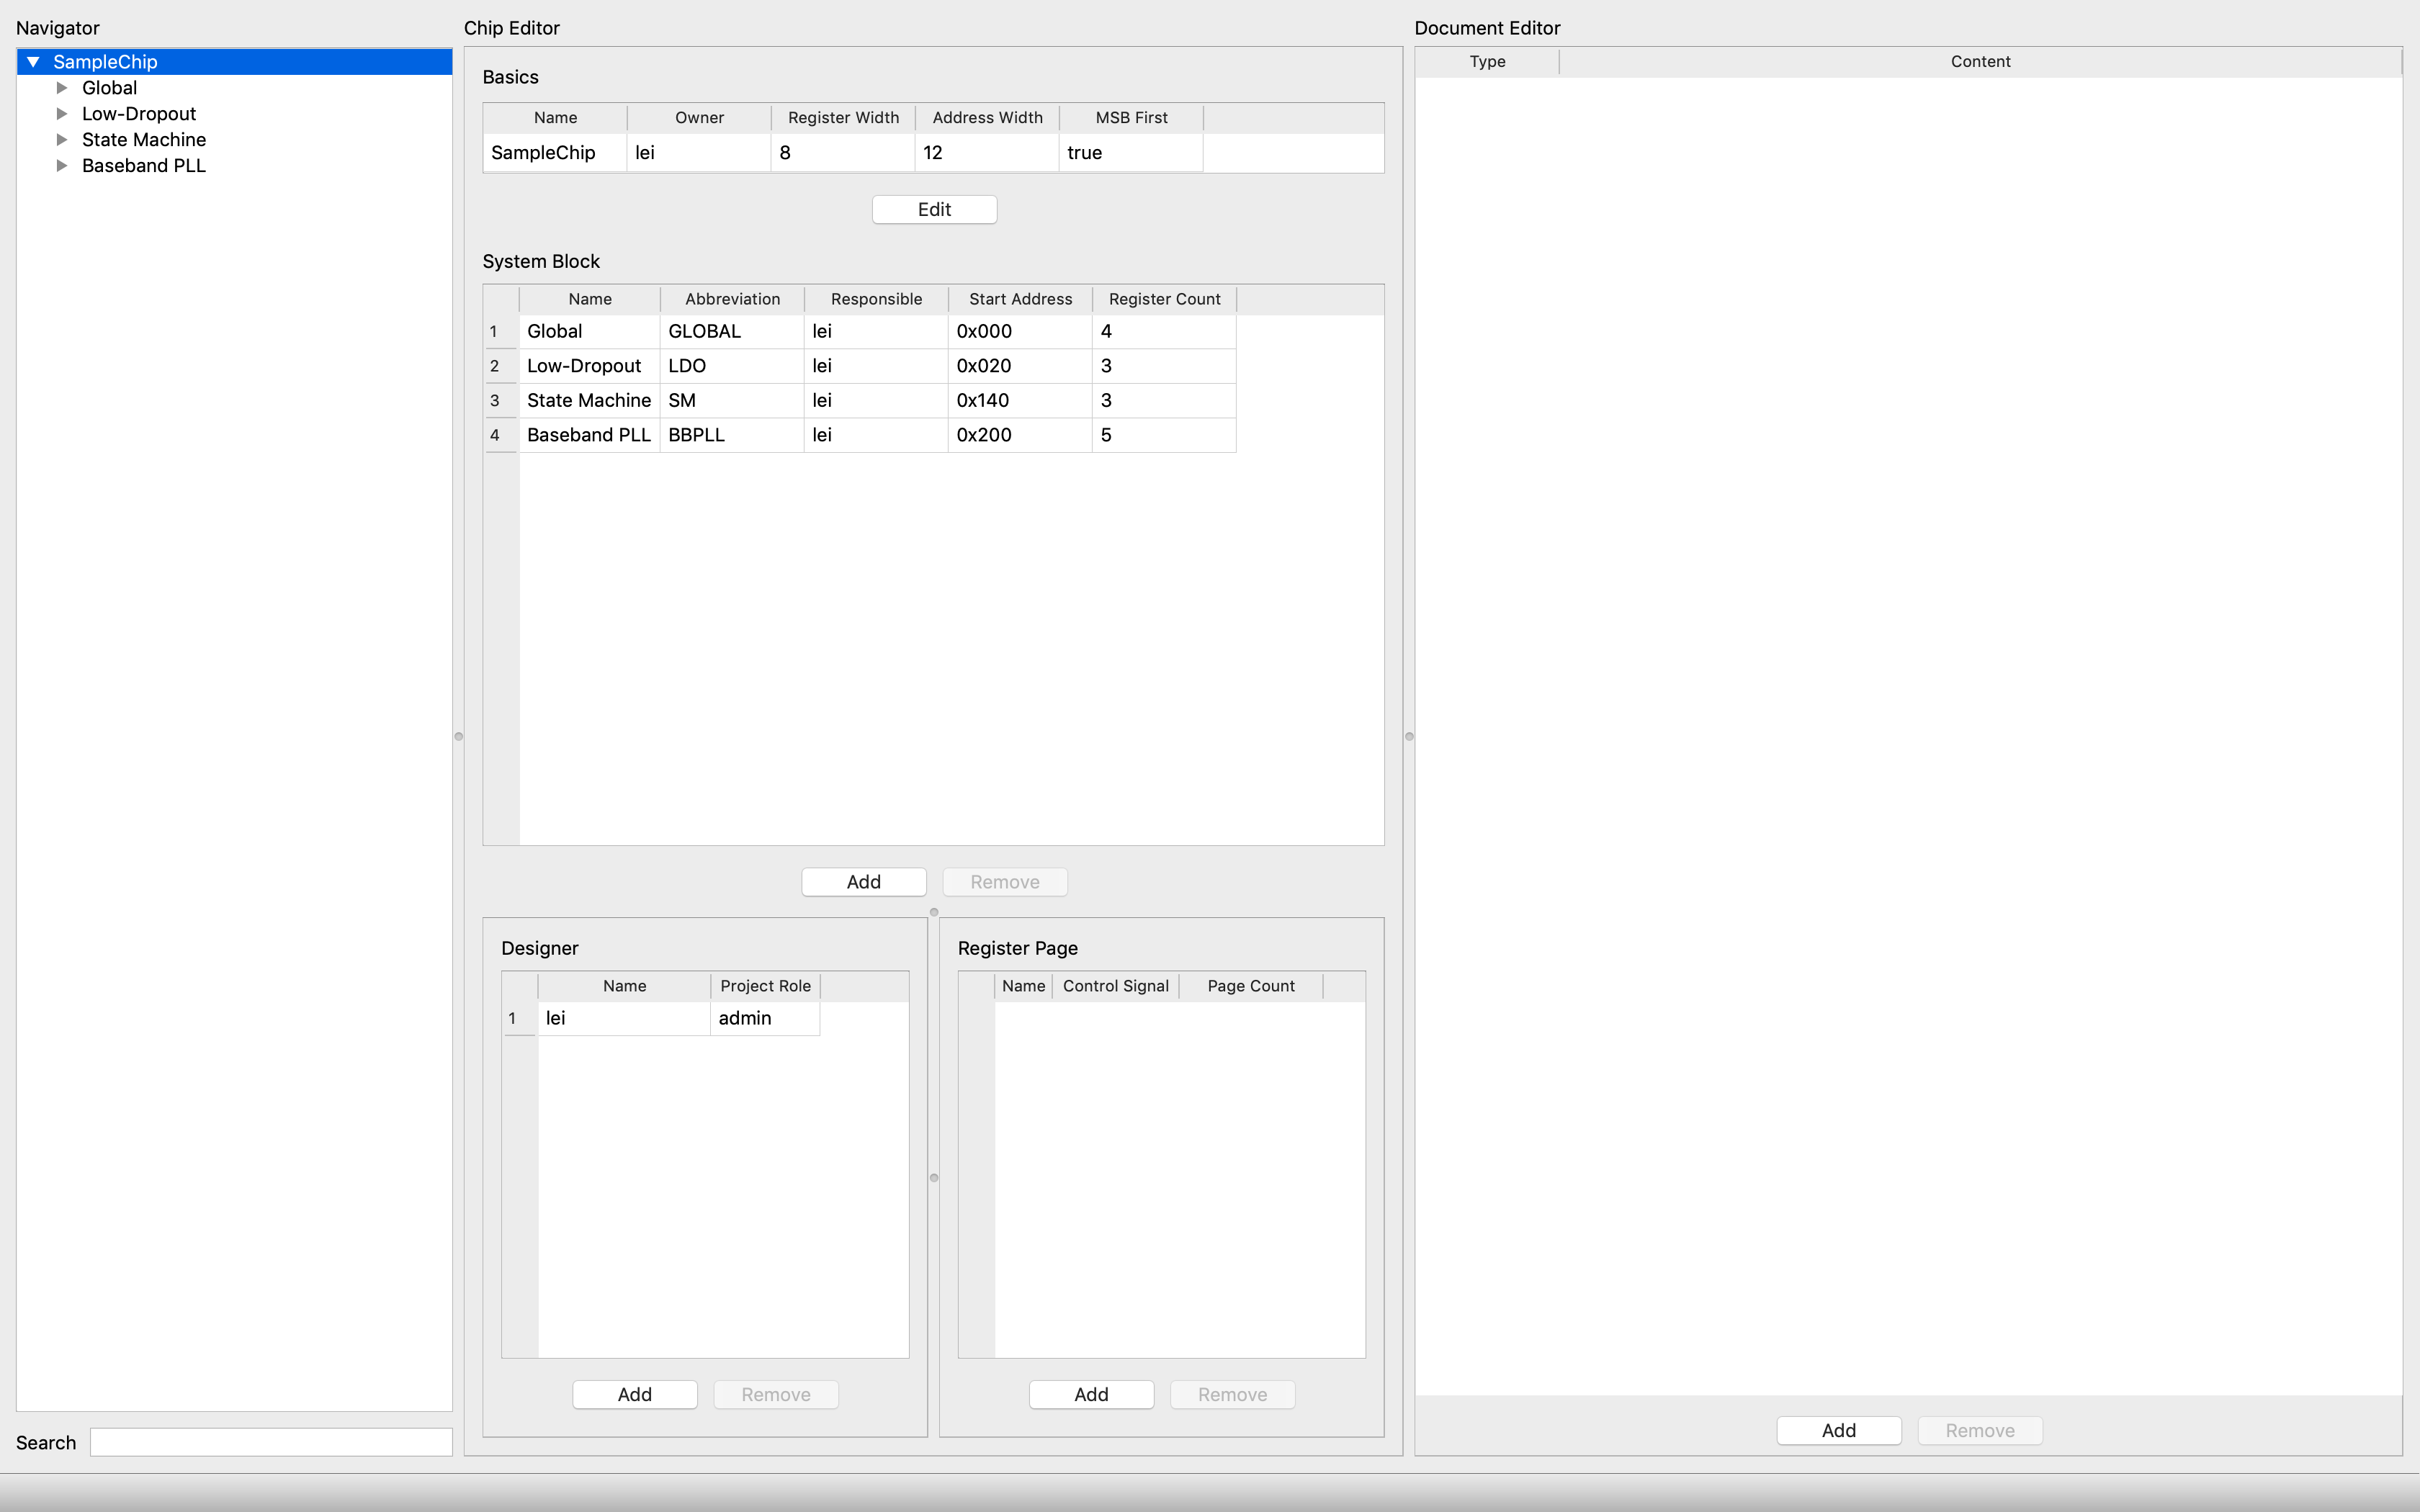
\includegraphics[width = \textwidth]{mainwindow}
\caption{Main Window\label{fig:Main Window}}
\end{figure}

We have described in the chapter Architecture Design how these components work together. When the current item of the ChipNavigator changed, the ChipEditorView and the DocumentEditorView have to respond. To make this happen, we defined a slot function in the ChipNavigator so as to deal with the predefined currentItemChanged() signal of the tree widget. According to the level of the current tree widget item, we know whether it is the chip, a system block, a register, or a signal. Then, we define signal functions for each level and emit them accordingly. The logic can be described by the following pseudo code.

\begin{lstlisting}[language=C++]
void  on_treeWidgetBlock_currentItemChanged(QTreeWidgetItem *current, QTreeWidgetItem *previous)
{
    if (level(current) == LEVEL::CHIP) 
        emit(chip_clicked());
    if (level(current) == LEVEL::BLOCK) 
        emit(block_clicked(get_block_id(current)));
    if (level(current) == LEVEL::REGISTER) 
        emit(register_clicked(get_block_id(current), get_register_id(current)));
    if (level(current) == LEVEL::SIGNAL) 
        emit(signal_clicked(get_block_id(current), get_signal_id(current)));
}
\end{lstlisting}

To take care of the signal, we defined slot functions in the RegisterManager class and connect them to corresponding signals. In the slot functions, we first update the current block, register and signal ID. Then, we reset the document level. We pass the IDs to the ChipEditorView and DocumentEditorView, then let them display documents and chip information respectively.

\begin{lstlisting}[language=C++]
// register_manager.h
void on_chipNavigator_chip_clicked();
void on_chipNavigator_block_clicked(QString block_id);
void on_chipNavigator_register_clicked(QString block_id, 
        QString reg_id);
void on_chipNavigator_signal_clicked(QString block_id,
        QString sig_id);
\end{lstlisting}

\begin{lstlisting}[language=C++]
// register_manager.cpp
void RegisterManager::on_chipNavigator_register_clicked(QString block_id, QString reg_id)
{
    ui->docEditorView->set_doc_level(LEVEL::REGISTER);
    ui->docEditorView->set_block_id(block_id);
    ui->docEditorView->set_register_id(reg_id);
    if (ui->frameDoc->isVisible() && ui->actionDocEditor->isChecked()) 
        ui->docEditorView->display_documents();

    ui->chipEditorView->set_block_id(block_id);
    if (ui->frameChipEditor->isVisible()) 
        ui->chipEditorView->display_system_level_info(reg_id);
    current_block_id_ = block_id;
    current_reg_id_ = reg_id;
    current_sig_id_ = "";
}
\end{lstlisting}

We can edit the chip in the ChipEditorView by editing the chip name, adding, editing or removing system blocks, registers, signals, signal-register mappings and so on. In these cases, the chip navigator have to be updated. Similarly, we define the following signals in the ChipEditorView, and corresponding slot functions in the RegisterManager. When the chip is edited, a certain signal is emitted and information is passed to the corresponding slot function in the RegisterManager. In the slot function, a certain function of the chip navigator is called so as to update the tree widget.

\begin{lstlisting}[language=C++]
// chip_editor_view.h
void chip_basics_edited(QString chip_name, 
                  QString chip_owner, 
                  QString chip_owner_id, 
                  int register_width, 
                  int address_width, 
                  bool msb_first);
void block_added(QString block_id, 
                  QString block_name, 
                  QString block_abbr, 
                  QString responsible);
void block_removed(int row);
void block_modified(int row, 
                  QString block_name, 
                  QString block_abbr, 
                  QString responsible);
void block_order_exchanged(int from, int to);
void to_refresh_block(); 
\end{lstlisting}

The boundaries between the ChipNavigator, ChipEditorView and DocumentEditorView are adjustable. Users can also switch on or off the ChipEditorView or the DocumentEditorView. 

We design a menu bar for the main window like this. There are 4 menus as follows, each containing a number of menu entries, or actions.
\begin{itemize}
\item User Menu \\
User Management: to open a UserManagementDialog in which users can add or remove users. It is only accessible to database admins. \\
Change Password: to open a ChangePasswordDialog. For users to change their password. \\
Log Out: to log out of the current user account and to login with another one. 
\item Chip \\
New Chip: to open an EditChipDialog to create a new chip. \\
New Chip From: to create a new chip from an existing one. \\
Open Chip: to open an OpenChipDialog and open the selected chip. \\
Close Chip: to close the current chip and clear everything in the ChipNavigator, ChipEditorView and DocumentEditorView. \\
Naming: to open a NamingTemplateDialog to either edit the naming for registers or signals. \\
Freeze/Unfreeze: to freeze or unfreeze the current chip. \\
Chip Management: to open an OpenChipDialog and configure it to the management mode. Users can add or remove chips. It is only accessible to database admins. 
\item Export \\
SPI Source Code: to open an SPIGenerationDialog and generate the SPI interface. \\
Document: to open an DocumentGenerationDialog and generate the document. 
\item View \\
Chip Editor: to enable or disable the ChipEditorView. 
Document Editor: to enable the Document Editor page of the DocumentEditorView. \\
Document Preview: to enable the Document Preview page of the DocumentEditorView. The Document Editor and Document Preview are exclusively checkable. 
\end{itemize}

\subsection{ChipNavigator}
We have described the logic of the main window and its interaction with the ChipNavigator, the ChipEditorView and the DocumentEditorView. The ChipNavigator is quite simple. According to requirements, the structure of the chip is represented with a tree widget of for level: CHIP-BLOCK-REGISTER-SIGNAL. The root of the tree is the chip level, with its children being system blocks. Under each system block are registers. The children of each register are those signals mapped to it.

We implemented a search mechanism which might be very beneficial especially when the chip is complex. The users can simply type in the pattern to search, and the tree widget will highlight those components containing that pattern and make the other invisible. The search process is written in a single search() function. Whenever the input pattern changes, the search() function will be executed in response to the textChanged() signal from the tree widget.

\begin{figure}[htbp]
\centering
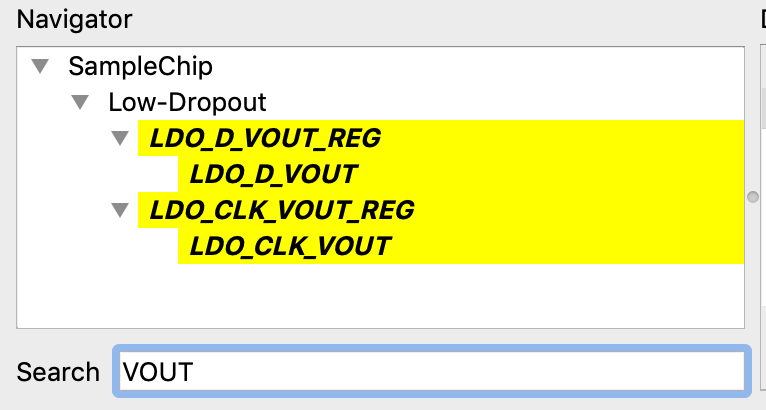
\includegraphics[width =0.5 \textwidth]{searchtree}
\caption{Chip Navigator: Search Example\label{fig:Chip Navigator: Search Example}}
\end{figure}

\subsection{Chip Editor View}
The ChipEditorView is one of the three major components of the main window. It displays information about the chip, and provides entrance to dialogs for editing the chip. According to the requirements, we designed the ChipEditorView as below.

\begin{figure}[htbp]
\centering
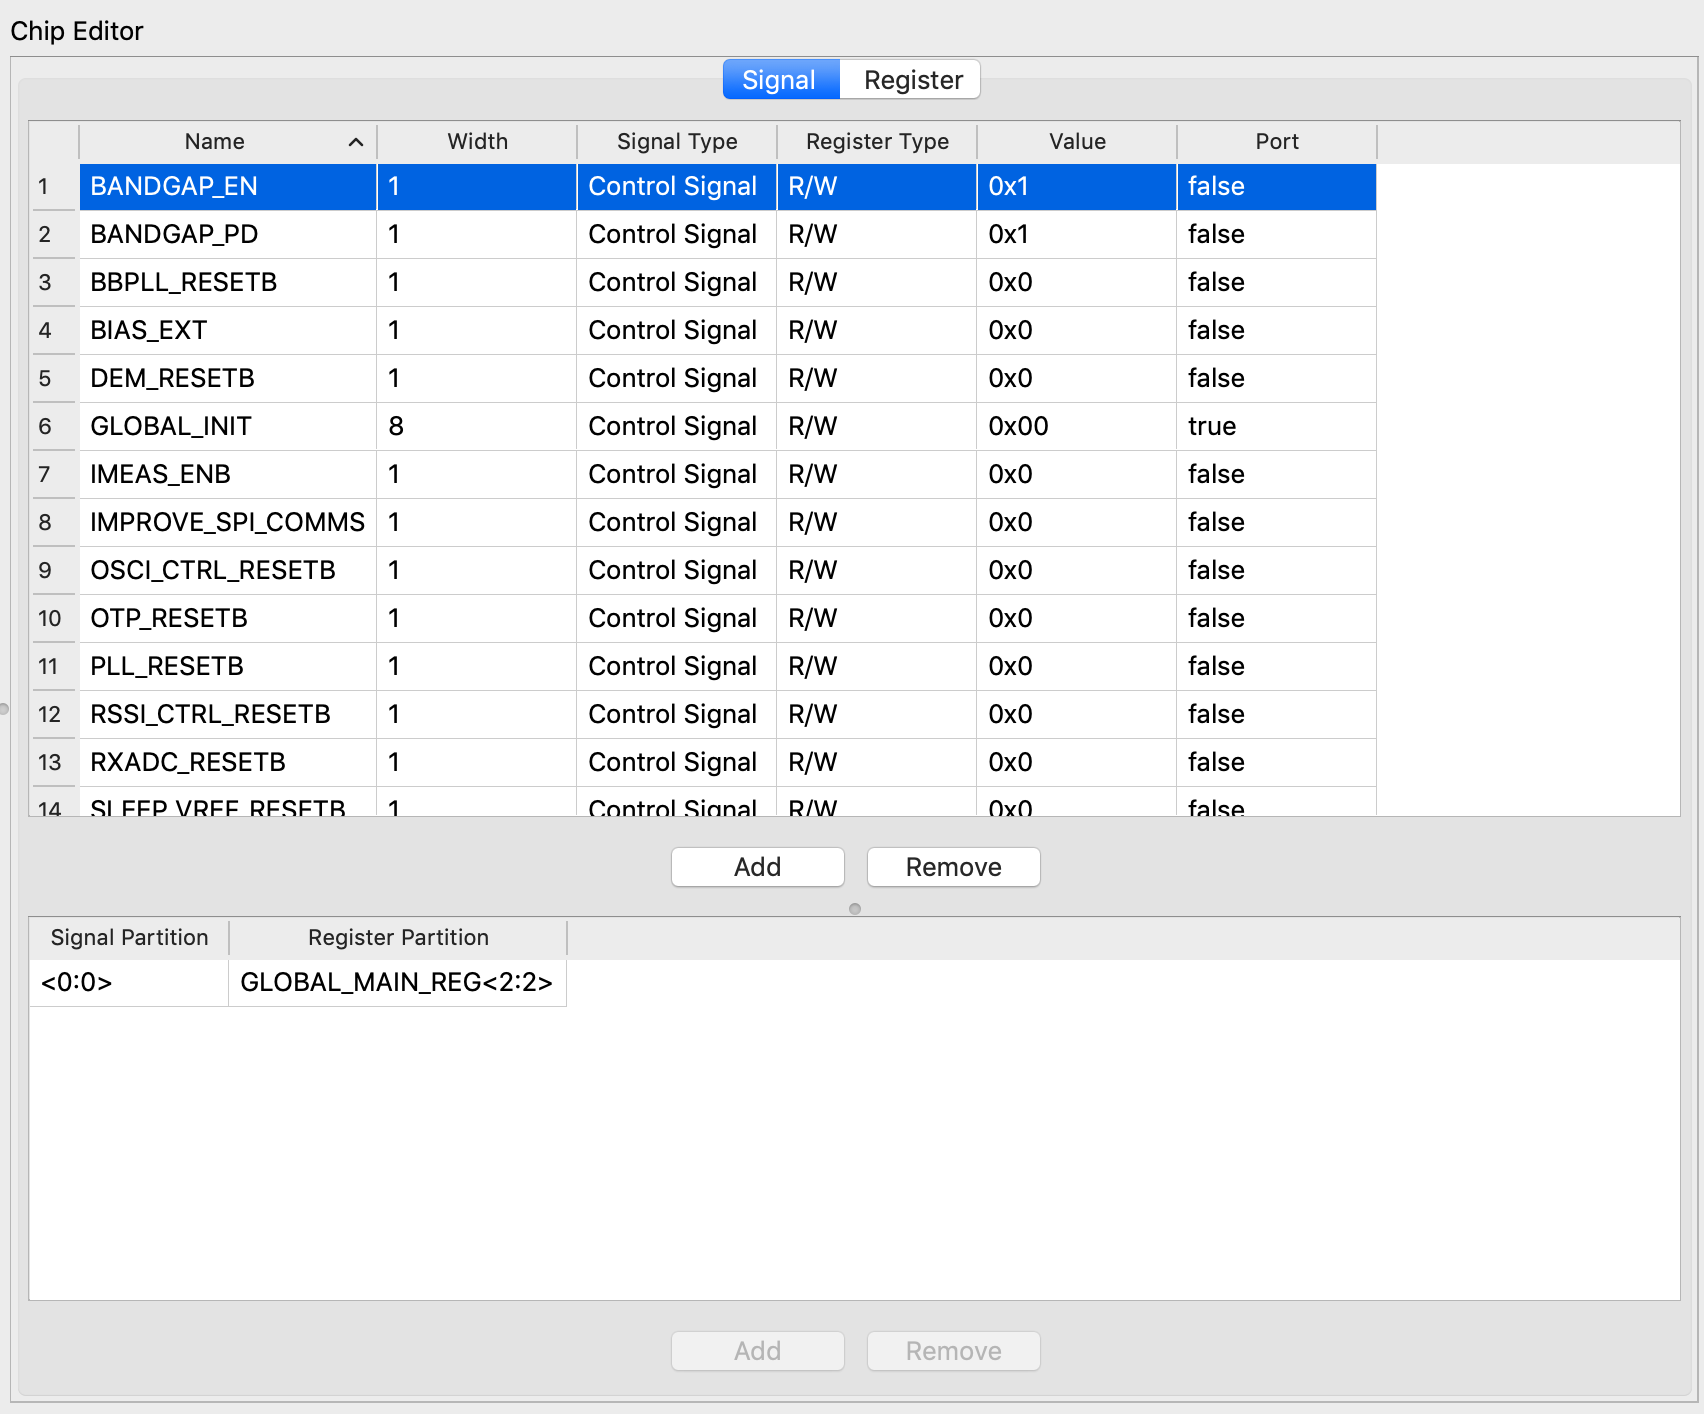
\includegraphics[width = \textwidth]{signalview}
\caption{Chip Editor: Signal Tab\label{fig:Chip Editor: Signal Tab}}
\end{figure}

\begin{figure}[htbp]
\centering
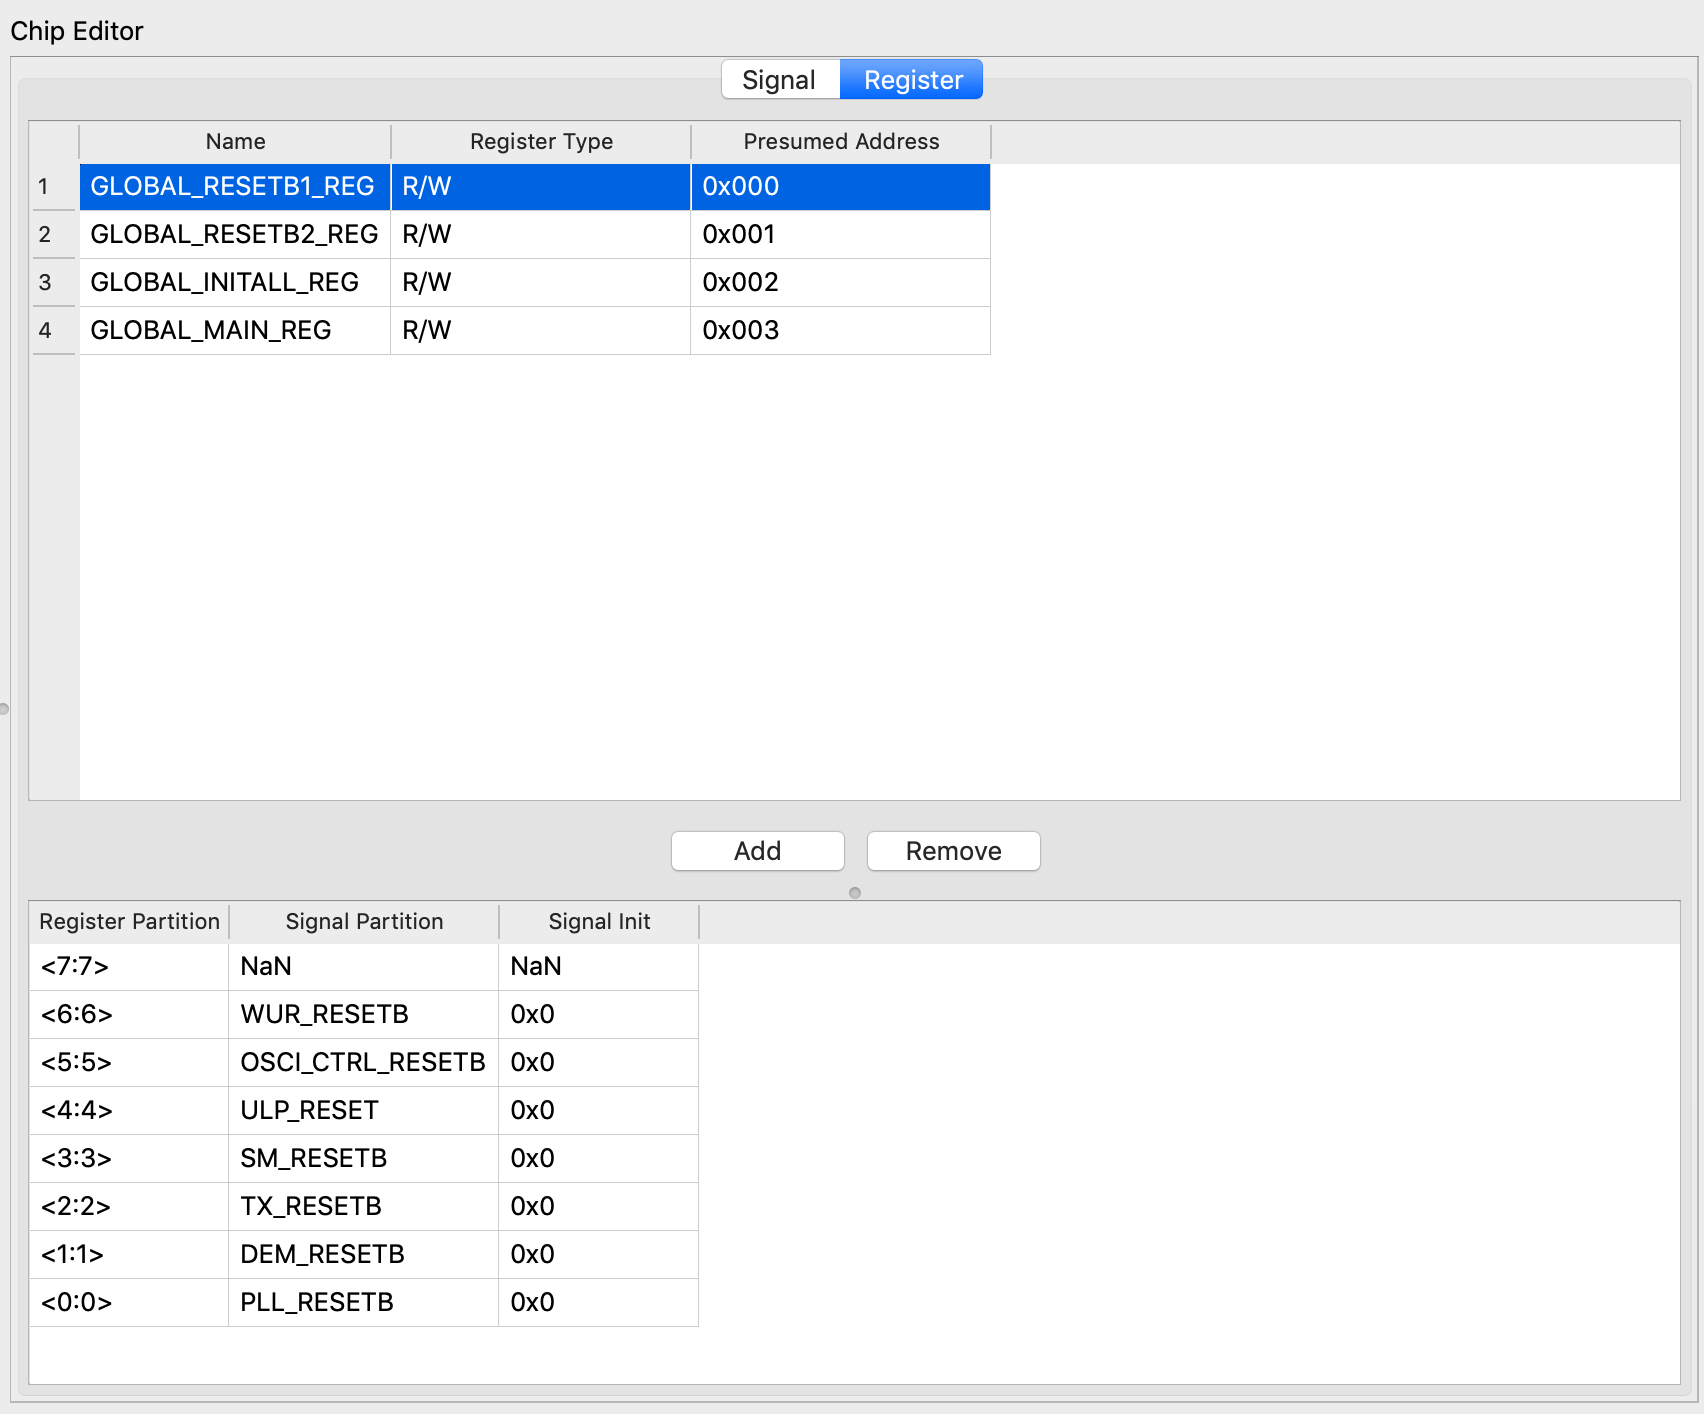
\includegraphics[width = \textwidth]{registerview}
\caption{Chip Editor: Register Tab\label{fig:Chip Editor: Register Tab}}
\end{figure}

Whether the chip level or the system level page is displayed depends on the current item of the navigator. If it is the root of the tree widget, then the RegisterManager class will call the display\_chip\_level\_info() function of the ChipEditorView, otherwise the display\_system\_level\_info(register\_id, signal\_id). If the current item is a register, then its register\_id will be passed to the function and signal\_id will be null. Likewise, if the item is a signal, then register\_id will be null. Depending on whether register\_id or signal\_id is null, the ChipEditorView will display the register page or the signal page, and set the selected register or signal in the register or the signal table as active. If the current item is a block, both register\_id and signal\_id are null, and the ChipEditorView simply displays the current page. This process can be described with the following simplified code.

\begin{lstlisting}[language=C++]
void ChipEditorView::display_system_level_info(const QString& reg_id, const QString& sig_id)
{
    // set to system level page
    ui->stackedWidgetChipEditor->setCurrentIndex(1);

    // set to register or signal page
    if (sig_id != "") ui->tabWidget->setCurrentIndex(0);
    else if (reg_id != "") ui->tabWidget->setCurrentIndex(1);

    // display either signals or registers
    if (ui->tabWidget->currentIndex() == 0) display_signals();
    else display_registers();
    
    // set current signal as active
    if (sig_id != "")
    {
        for (int row = 0; row < ui->tableSignal->rowCount(); row++)
            if (sig_id == ui->tableSignal->item(row, 0)->text())
            {
                ui->tableSignal->setCurrentCell(row, 0);
                break;
            }
    }
    // set current register as active
    else if (reg_id != "")
    {
        for (int row = 0; row < ui->tableRegister->rowCount(); row++)
            if (reg_id == ui->tableRegister->item(row, 0)->text())
            {
                ui->tableRegister->setCurrentCell(row, 0);
                break;
            }
    }
}
\end{lstlisting}

To add a system block, register, signal or a signal-to-register mappings we provide a push button under each table. After a click on the button a dialog of the corresponding class will be created and open. To remove an existing item we can click on the Remove buttons leading to execution of a corresponding slot function. The function will first remove the system block, register etc in the database, then remove it from the table. To edit an existing system block, register or signal, we can double click the table entry. The cellDoubleClicked() signal will then be emitted. We write corresponding slot functions to help us edit the items. The logic is actually very similar to adding a new item. A corresponding dialog will open, but the it will be initialized with data related to that item. The dialogs will be discussed in the later sections. 

For users' convenience, we designed a right-click context menu containing an Edit, Remove and Add action. Users do not have to click on the push buttons below each table. The menu also contains a Refresh action, which allows for reloading data from the database and refreshing the table. Once we right-click on the tables, a customContextMenuRequested() signal will be triggered. A slot function is then called to display the context menu in response to the signal.

\subsection{Document Editor View}
The DocumentEditorView is another central component of the software. It displays documents and provides entrance to editing the documents. According to the requirements, it should contain a table widget showing documents of the current item on the chip navigator. At the bottom of the DocumentEditorView there is an editing "dialog" in which we can add or edit a document. It is an instance of the EditDocumentDialog class, which is not a real dialog though, but a subclass of the generic QWidget. This is because the QDialog cannot be a child widget of another one. The dialog can be switched on or off. Like the ChipEditorView, we can add or edit documents by clicking on the Add button below or double clicking a table entry. The editing dialog will then open. If we finished editing and want to save the document, we click on the Ok button. The document will be saved to the database and the table above will be updated. Then, the editing area will be switched off. If we want to abandon the document we are editing, simply click on the Cancel button. 

\begin{figure}[htbp]
\centering
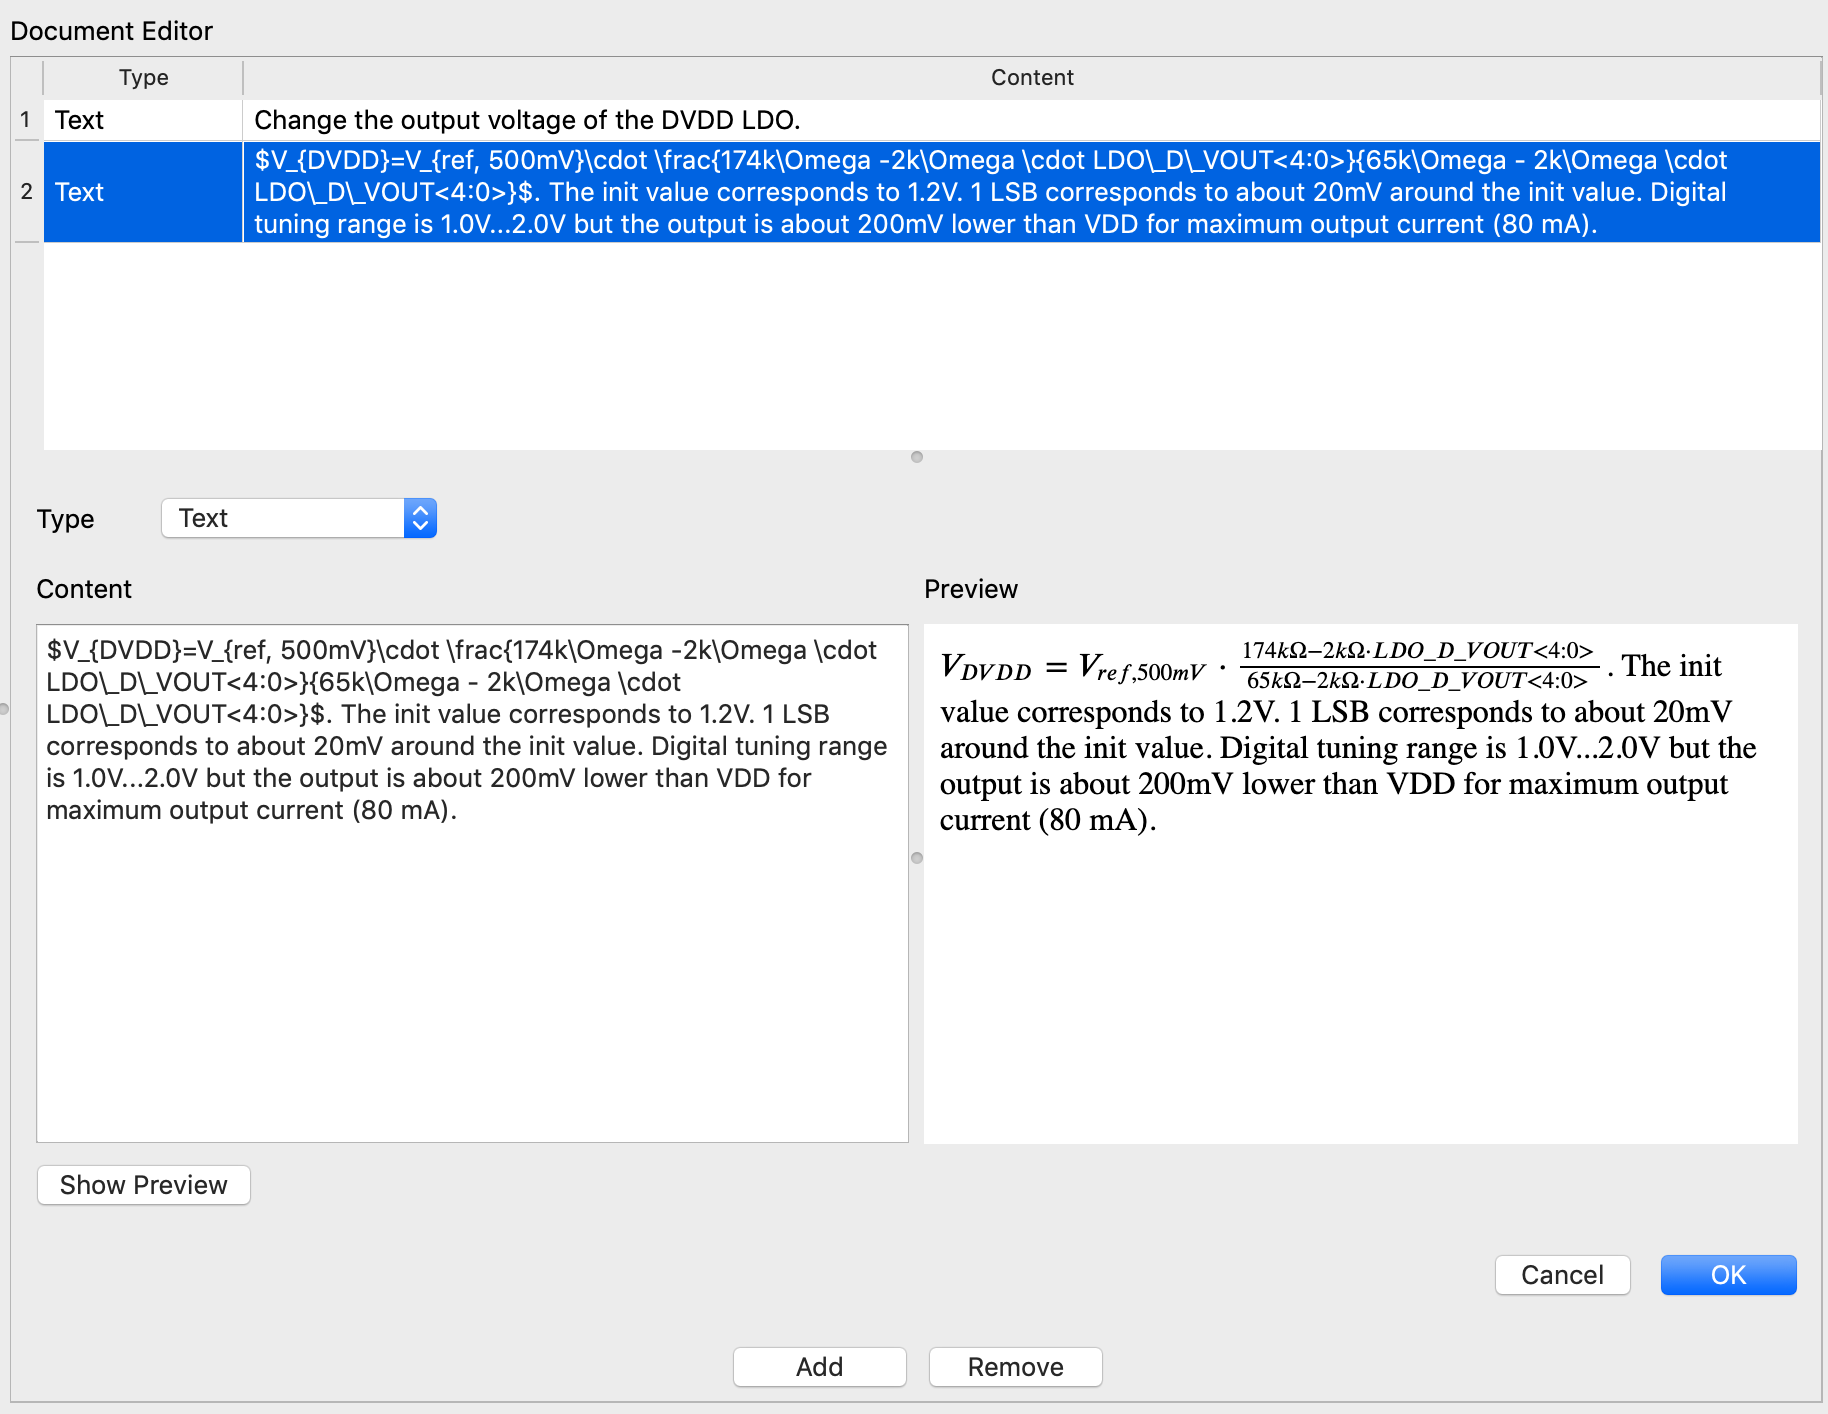
\includegraphics[width = \textwidth]{documentview}
\caption{Document Editor View\label{fig:Document Editor View}}
\end{figure}

Apart from the Add, Remove and Edit functions, we provided a copy and paste mechanism, which might be very useful for documentation editing. To achieve this, we maintain a member variable copied\_ of type QString. When we copy a document, the corresponding document type ID, document type, and the content to copy will be concatenated by a special delimiter and then be stored in this copied\_ variable. When we paste the copied content, the copied\_ variable will be parsed to fetch the document type ID, document type, and the content to paste. With this information, we can create a new entry in the document table and store this document to the database.

\section{Chip and Document Editor Dialogs}
To edit chip components and documents, we have to design different dialogs encapsulating both UI and business logics. These dialogs are named after EditSomethingDialog, such as EditChipDialog and EditSignalDialog. Their definitions follow the framework.

\begin{lstlisting}[language=C++]
class EditSomethingDialog : public QDialog
{
    Q_OBJECT

public:
    explicit EditSomethingDialog(QWidget *parent = nullptr);
    explicit EditSomethingDialog(QString something_id, bool enabled, QWidget *parent = nullptr);
    // other construction functions
    ~EditSomethingDialog();
    QString get_something_id();
    // Other public functions
    
    bool add_something();
    bool edit_something();

private:
    bool setup_ui();
    void accept(); // override QDialog::accept()
    bool sanity_check();
    /*
     Things to check
    */
    // Other private functions

    Ui::EditSomethingDialog *ui;
    const bool enabled_;
    const DIALOG_MODE mode_;
    QString something_id_;
    // Other private member variables 
};
\end{lstlisting}

The class has at least two construction functions, one for adding, the other for editing something. The DIALOG\_MODE mode\_ will correspondingly set to ADD or EDIT. Upon construction the dialog first setup the UI by calling the setup\_ui() function. If the dialog is constructed in the EDIT mode, it will pass the ID to the dialog and fill in the existing data into the widgets. Also, there is a parameter called enabled. If it is false, then the UI components will be disabled so users cannot put in anything to the dialog. Otherwise, users give their input to the dialog and click on the Ok button, and the accept() function will be executed. 

By default, if the EditSomethingDialog is executed as modal, the QDialog::accept() function will close the dialog and its exec() function will return QDialog::Accepted. However, we override the QDialog::accept() as below.

\begin{lstlisting}[language=C++]
void EditSomethingDialog::accept()
{
    if (!enabled_) return QDialog::reject();
    if (sanity_check()) return QDialog::accept();
}
\end{lstlisting}

If the dialog is not enabled, then just reject. This is equivalent to clicking on the Cancel button. Otherwise, do sanity check, which one of the system requirements. If the check is successful, then accept, else do nothing to the dialog. The purpose of the sanity check is to determine whether the input data is valid. The sanity\_check() function might be similar to

\begin{lstlisting}[language=C++]
void EditSomethingDialog::sanity_check()
{
    return check1() && check2() && check3();
}
\end{lstlisting}

We can determine what we want to check. The checking functions are defined like the example below. They basically follow the same pattern. They check something, prompt error message and return false at once if a check failed, or return true if all checks passed. In this example, we want to verify if the name is valid. The name must not empty or duplicate. If it is empty, a warning message will be prompted and the function will return false. Otherwise, if you are in the ADD mode, we have to fetch names from the database and check if the name already exists. If so, users are warned and the function returns false. If everything was fine, then return true. It is a little different in the EDIT mode. In that case, the original name actually exists in the database. If the current updated name equals the original name, the function just returns true, otherwise we check it as in the ADD mode.

\begin{lstlisting}[language=C++]
bool EditSomethingDialog::check_something_name()
{
    QString name = get_something_name();
    if (name == "")
    {
        QMessageBox::warning(this, "Add Something", "Something name must not be empty!");
        return false;
    }
    if (mode_ == DIALOG_MODE::EDIT && name == original_name_) return true;
    if (exists_in_database(name))
    {
        QMessageBox::warning(this, "Add Something", "Something" + name + "already exists!")
        return false;
    }
    return true;
} 
\end{lstlisting}

If the exec() function returns true, we then execute either the add\_something() or edit\_something() function. Then, we get what data we need from the dialog. We use the dialog to add or edit something as below.

\begin{lstlisting}[language=C++]
// add something
EditSomethingDialog add_somthing(this);
If (add_somthing.exec() == QDialog::Accepted && add_somthing.add_something())
{
    QString something_id = add_somthing.get_something_id();
    // Other data we want to get
    // Do something
}

// edit something existing
QString something_id; // got from somewhere
bool enabled; // got from somewhere
EditSomethingDialog edit_somthing(something_id, enabled, this);
If (edit_somthing.exec() == QDialog::Accepted && edit_somthing.edit_something())
{
    // Other data we want to get
    // Do something
} 
\end{lstlisting}

The most complex editor dialogs are the EditSignalDialog and EditDocumentDialog. The EditSignalDialog allows users to add or edit signals. Users have to put in the signal name, width or number of bits, signal type and whether to add a port for this signal. If the signal is writable, users have to put in its initial value. If the signal can be mapped to a register, or in other words, it is a register-signal, the dialog allows users to edit signal-register mappings. A signal can only be mapped to one type of registers.

In practice we found almost half of the signals are single-bit signals. In this case, the signal cannot be partitioned. It can be mapped to a certain bit of a register as a whole. In other cases where the signal have more bits, we might want to partition the signal, and map the signal partitions to certain registers partitions. We therefore design UI for two cases. In case of a single-bit signal, users just need to select a certain register and a certain bit of it to map the signal to. Users don't have to explicitly add a signal-register mapping to the partition list. In case of a multi-bit signal, however, users must determine the signal partition, select a register, and a register partition. Then, add the partition to the candidate list. Of course, users can also remove signal-register mapping from the candidate list. To make it more user friendly, we can add a new register by clicking on the button beside the register combo box.  

\begin{figure}[htbp]
\centering
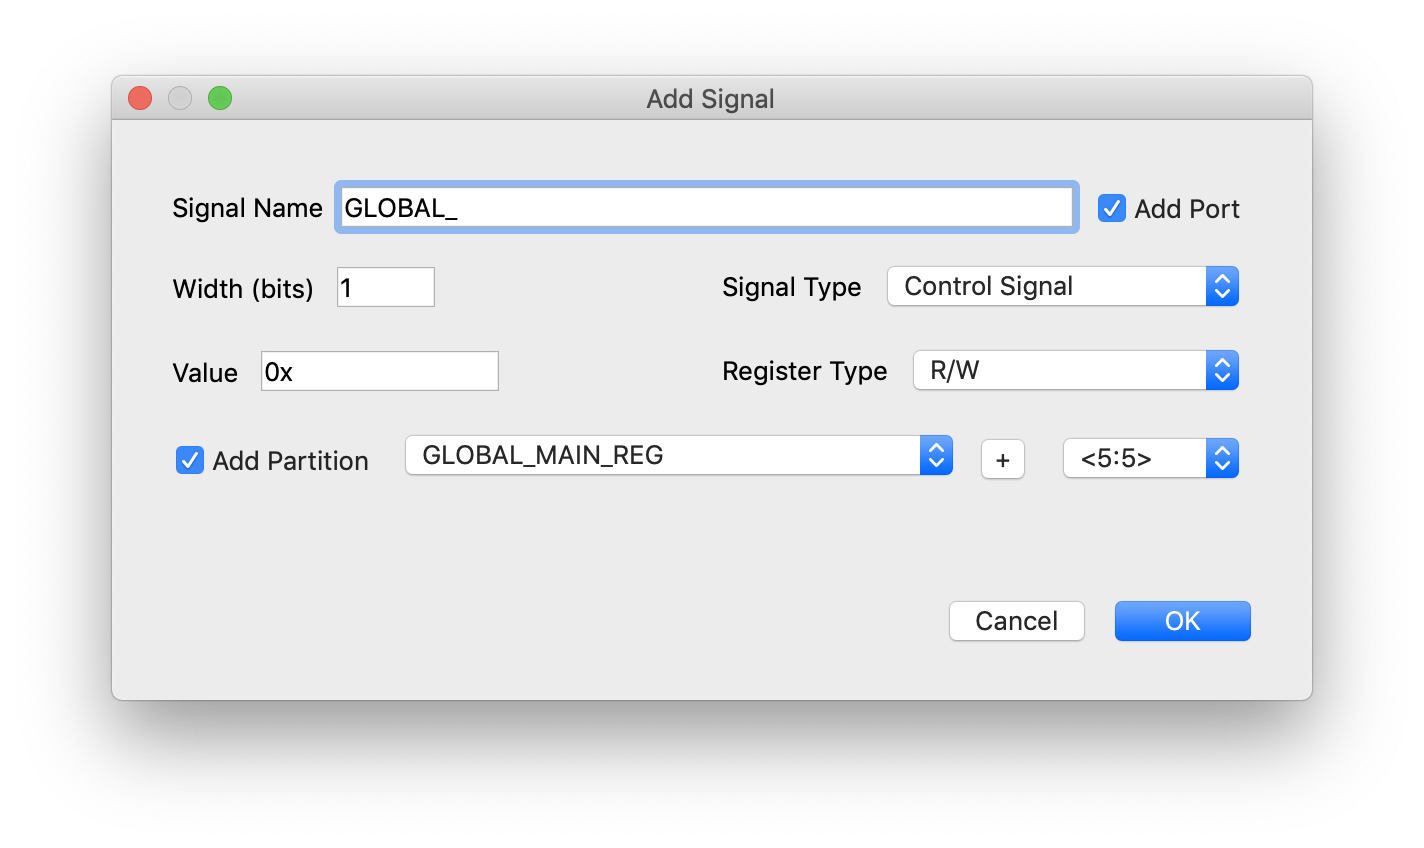
\includegraphics[width = 0.8 \textwidth]{singlebitsignal}
\caption{Single-bit Signal\label{fig:Single-bit Signal}}
\end{figure}

\begin{figure}[htbp]
\centering
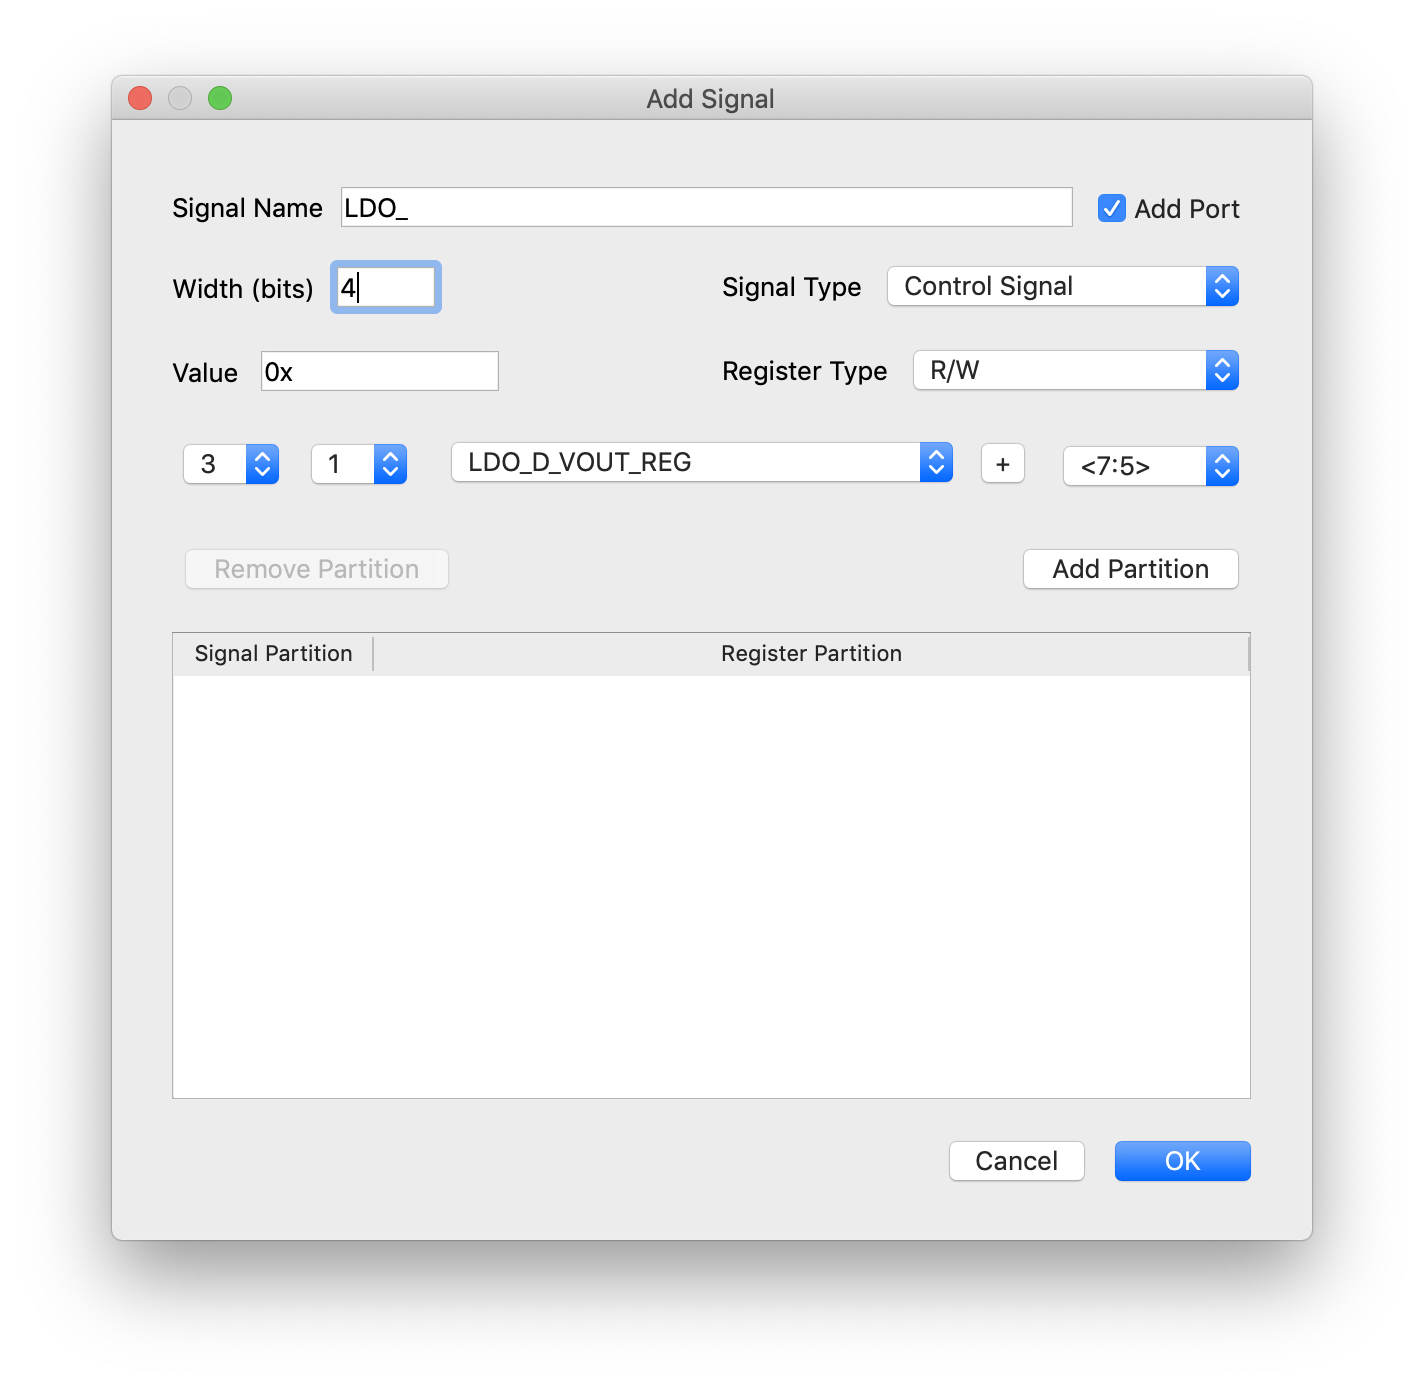
\includegraphics[width = 0.8 \textwidth]{multibitsignal}
\caption{Multi-bit Signal\label{fig:Multi-bit Signal}}
\end{figure}

Widgets in the EditSignalDialog have pretty strong interaction with each other. Whenever the signal width changed, the signal-register mappings might be invalid, thus we have to clear the candidate list. Also, we have to adjust the UI according to the signal width. If the signal type changed, we have to retrieve from the database the register types available to such signal type, and change items in the register type combo box. If the current register type changed, we have to clear the signal-register mapping candidate list, and retrieve registers of such type from the database. Whenever the candidate list changed, we also have to find available signal partitions. It is crucial that a signal bit cannot be mapped to more than one register bit, and the other way around. The register partition combo box changed according to the signal LSB and MSB combo boxes. The signal/slot technique provided by Qt makes these changes much more tractable.

The EditDocumentDialog allows users to add documents to the current item in the ChipNavigator, or edit existing ones. It is named after dialog but it is actually not one, because we want to incorporate it in the DocumentEditorView, and this is not possible for a dialog. Instead, it is a subclass of QWidget. However, we design it totally following the the pattern of the editor dialogs.

We defined three document types, text, image and table. Thus, the EditDocumentDialog is designed so that it can take in all document types. To make this possible the dialog has a stacked widget containing three pages, each handling a document type. In the previous section the DocuementEditorView example has already shown the page for text document. Below are image page and table page.

\begin{figure}[htbp]
\centering
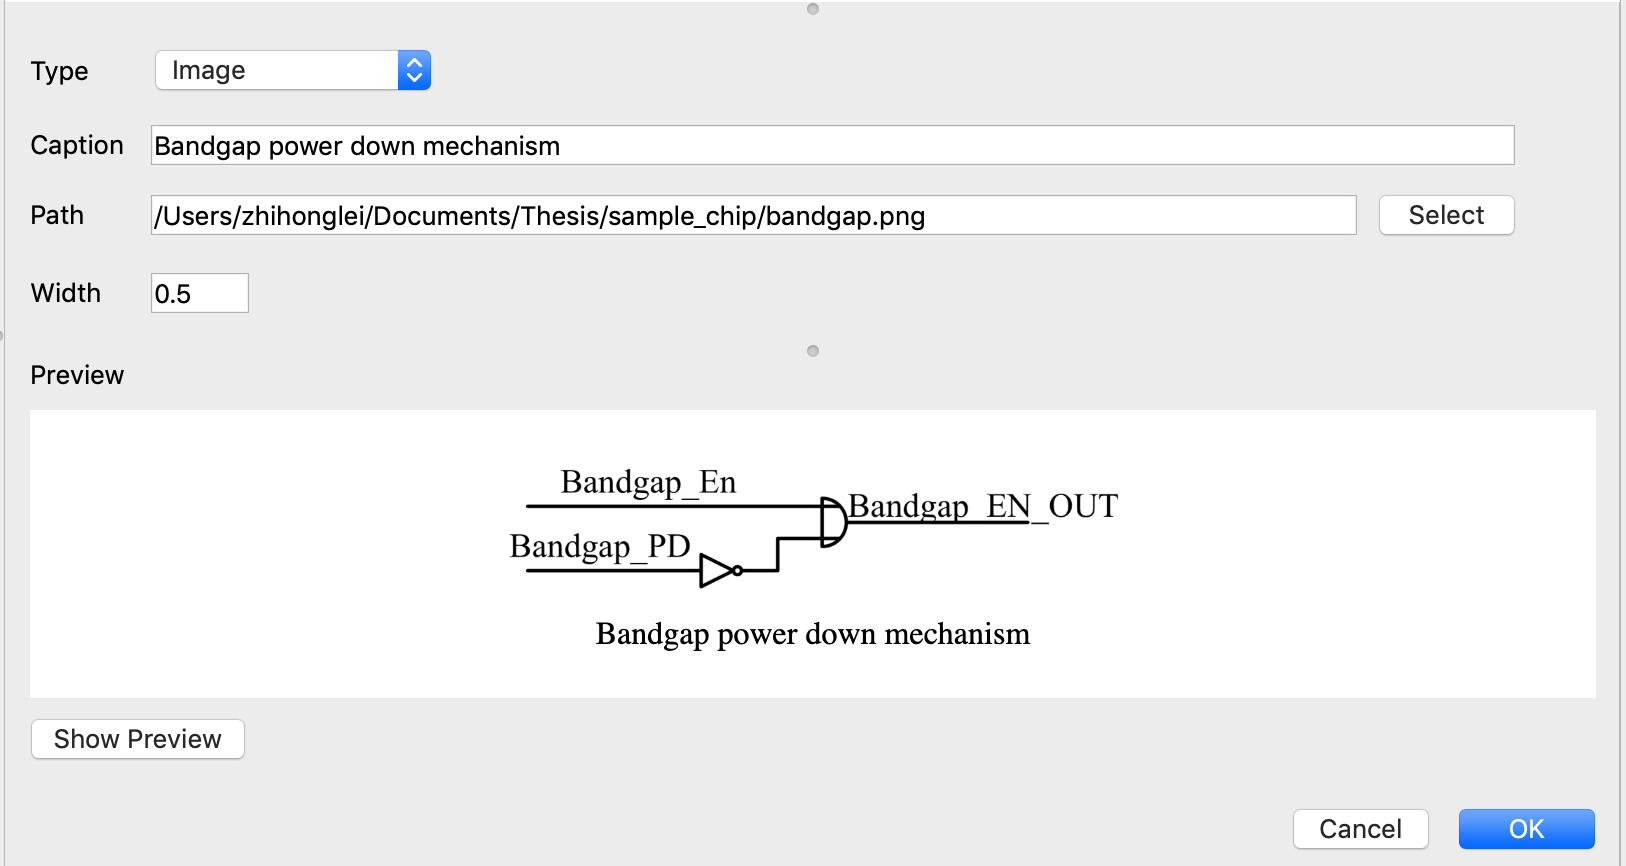
\includegraphics[width = \textwidth]{imagedoc}
\caption{Image Document\label{fig:Image Document}}
\end{figure}

\begin{figure}[htbp]
\centering
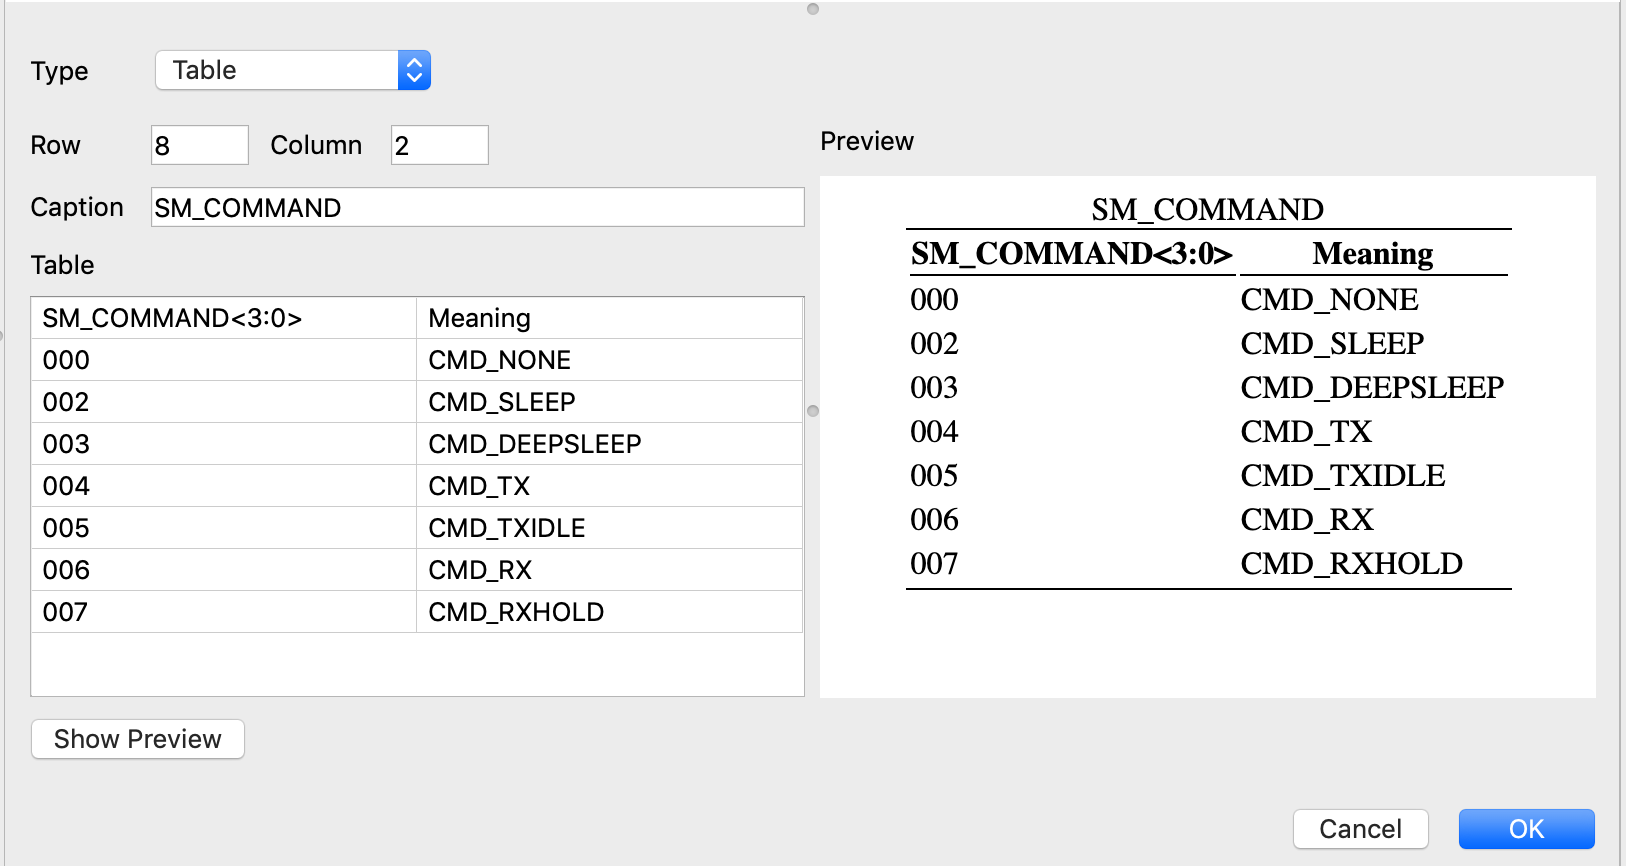
\includegraphics[width = \textwidth]{tabledoc}
\caption{Table Document\label{fig:Table Document}}
\end{figure}

The text page has a QPlainTextEdit, in which we can edit multiple lines of text. In the image page, we can specify a caption of the image, select an image in a QFileDialog and get its path. It is also important to specify how large the image is in terms of page width. The number can vary between 0 and 1. In the table page, there is a QLineEdit holding the caption of the table. There is a QTableWidget in which we can edit the table contents. We can specify number of rows and columns for the table.

We will store the document in the database. The question is how to deal with different types of documents. The text document is simple. We just store the text in the database. For image documents, our solution is to concatenate the caption, width, and the path with a special delimiter, and store the concatenated string in the database. Similarly, for the table document, we concatenate the caption, row count, column count, and all cell contents. In this solution, of course the image caption, table caption and cell contents must not contain the delimiter. It would be a good idea to use a very rare string as the delimiter. We can easily restore the documents in a reverse way.

It's inevitable that we might have to include math equations in LaTeX format in the documents. In this case, of course we can type LaTeX code "blindly". It would be very nice if we have a preview of the LaTeX math equations. In this way, the input is more visual, and we can check if the code is correct. We also want to have a preview of the table and image. It's important that table cell contents can also contain LaTeX math equations.

To implement the preview, we might want to compile the LaTeX source code to generate a PDF document. Then, we must find a way to display the PDF document in our software. This is not a good idea. First, users have to install a LaTeX compiler on their machines and it must be accessible to the software. Second, Qt does not have a PDF render. We were able to find third-party renders, but they are either of low quality or hard to incorporate in our software.

However, we found MathJax, a JavaScript display engine for mathematics that works in web browsers. With MathJax included in the HTML web page, LaTex source code can be simply inserted in the HTML code, and browsers can render it properly. We use MathJax with the following template.

\begin{lstlisting}[language=HTML]
<!-- HTML template -->
<html>
<head>
    <script type="text/x-mathjax-config"> MathJax.Hub.Config({
        tex2jax: {inlineMath: [['$','$'], ['\\(', '\\)']]}});</script>
    <script type="text/javascript" src="MATHJAX_ROOT/MathJax.js"></script>
</head>
<body>
HTML_CONTENT    <!-- write your HTML code here -->
</body>
</html>
\end{lstlisting}

Inspired by this, we can display text, image and table documents in a web browser. For text documents it is quite simple. We just replace HTML\_CONTENT in the HTML template with the text in the text editor. For image and table documents, we created a template respectively. Using the image or table template, we generate image or table HTML source code, and replace HTML\_CONTENT in the HTML template.

\begin{lstlisting}[language=html]
<!-- HTML image template -->
<style>
    figure img {display: block; margin-left: auto; margin-right: auto;}
    figure figcaption { text-align: center;}
</style>
<center>
<figure>
   <img style='width: WIDTH; object-fit: contain' src="IMAGE" alt="CAPTION"/>
    CAPTION
</figure>
</center>
\end{lstlisting}

\begin{lstlisting}[language=html]
<!-- HTML table template -->
<style>
    table {border-top: 1px solid black; border-bottom: 1px solid black}
    th {border-bottom: 1px solid black}
    caption#tab {caption-side: CAPTION_POS}
</style>
<center>
<table>
TABLE
</table>
</center>
\end{lstlisting}

Fortunately, Qt provides a web engine based on Chromium. Thus, we are able to make a preview based on the web engine. The preview is intrinsically a web browser. To display documents of any types, we generate the HTML source code and fill it into the browser. In this way, the document editor can display the real time preview of the text we are editing.

Another effort we made is to implement an auto-completer. This is especially useful for editing text documents. The completer we designed takes all system block names, system block abbreviations, register names and signal names as candidates. Besides these, the software allows users to extend the word list by simply add txt files containing candidate words to the \textbf{completion} directory under the root directory of the software.

\begin{figure}[htbp]
\centering
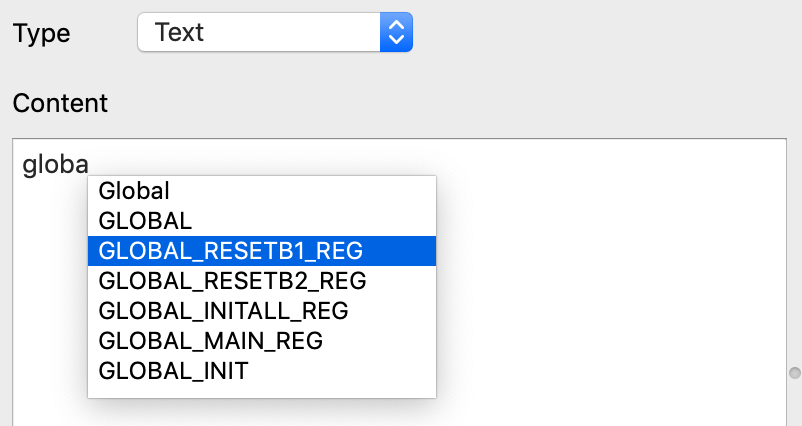
\includegraphics[width = 0.5\textwidth]{completer}
\caption{Document Completer\label{fig:Document Completer}}
\end{figure} 

\section{User Account, Authentication and Password}
For data security reasons, the software is required to provide user access control and authentication. User access control has two levels, the software level or the database level, and the project level. If a user account is created, the user can log in to the software with this account. However, it does not necessarily mean he or she has access to a certain chip. This is controlled by the project level permissions.

All users must have access to the database, thus, we need to establish database accounts for them. MySQL provides a very good user account management. We can grant different permissions for different user. However, the permissions we want to implement are more complex. For example, in a certain table, a user might have access to row A but not to row B. This is not possible with MySQL. Thus, we have to manage permissions using our software. In this background, we distinguished the software account and database account. We store user accounts in the database. Users log in to the database using a shared database account, retrieve user account information and determine if they have access to the software. Similarly to the user account, chip designers, database level and project level permissions are also stored in the database.

We define different database permissions allowing users to add or remove users, add or remove projects. A special permission is reserved for the database/software admins, so they have full access to all projects. This means that they can do anything on any projects, even if they are in the designer list of those projects. We predefined two database roles, the admin and standard user. However, we can extend the database roles without modifying the software. Similarly, we defined different project permissions allowing chip designers to add system blocks, remove the system blocks they are in charge of, read all system blocks, add or remove chip designers.

To make use of the database and project permissions, we designed an Authenticator class. To make block level authentication more manageable, we also defined block permissions here. They are determined by project permissions and the responsible person of the system block. The Authenticator class allows users to set database permissions, project permissions and block permissions. The permissions are stored member variables db\_permissions\_, project\_permissions\_, block\_permissions\_ of data type int. Each bit of the permissions variable represents a permission, which is defined in the enumeration DATABASE\_PERMISSIONS, PROJECT\_PERMISSIONS, and BLOCK\_PERMISSIONS. We set or get permissions using bit operations. For example, to set ADD\_USER permission, we make the 0th bit of db\_permissions\_ be 1. To get ADD\_USER permission, we get the value of the 0th bit of db\_permissions\_.

\begin{lstlisting}[language=C++]
class Authenticator
{
public:
    enum DATABASE_PERMISSIONS
    {
        ADD_USER = 1 << 0,
        // ...
        FULL_ACCESS_TO_ALL_PROJECTS = 1 << 4
    };
    // enum PROJECT_PERMISSIONS
    // enum BLOCK_PERMISSIONS
    
    Authenticator(const QString& db_role_id, const QString& project_role_id);
    Authenticator();

    void set_database_permissions(const QString& db_role_id);
    void set_project_permissions(const QString& project_role_id);
    void set_project_permissions(bool setting);
    void set_block_permissions(bool setting);
    void freeze(bool frozen=true);

    // database permissions
    bool can_add_user() const;
    // ...
    bool can_fully_access_all_projects() const;

    // project permissions
    bool can_add_block() const;
    // ...
    bool can_fully_access_all_blocks() const;
    
    // block permissions
    bool can_add_signal() const;
    // ...
    bool can_edit_document() const;
    
    bool frozen() const;

    void clear_database_permission();
    void clear_project_permission();
    void clear_block_permission();
    void clear_all_permission();

private:
    int db_permissions_ = 0, project_permissions_ = 0, block_permissions_;
    bool frozen_;
};
\end{lstlisting}

We provide a convenient way for managing user accounts using the UserManagementDialog. It allows database admins to add or remove users. To add a user, we need the CreateUserDialog. We specify the username, initial password and select a database role. Like the editor dialogs, we have to check whether the username is valid. After creation of a user account, users can then log in to the software using the account. To remove a user, however, it will be tricky. The users to be deleted might be the owner of some chips. They might be a designer in some chips, and responsible for some system blocks. In this case, our solution is to replace the users in those chips with the database admin who is deleting these users. Users can change their passwords easily using the ChangePasswordDialog.

On the project level, designers can be added to a chip with the EditChipDesignerDialog, where a user and a project role are selected. Before adding a designer, the dialog shall check whether the selected user already exists in the current chip. We can also delete a chip designer. Like removing a user, the software has to replace the designers in this chip with a project admin.

As previously described, the software account and database account are not the same. In our solution, all software users share a single database account. The problem is that we don't want users to know the password to the database to prevent them from bypassing the software and directly work on the database. This might cause serious data security problems.

Our solution is to introduce an encryptor and decryptor. We designed an encryption class using the AES algorithm. The encryptor can encrypt a plain password with a key. With this key and encrypted password, the decryptor can generate the original plain password. Only the admins know the password. They generate encrypted password, and give users the key and the encrypted password instead of the original password. We made a tool for admins to make encrypted passwords easily.

\begin{figure}[htbp]
\centering
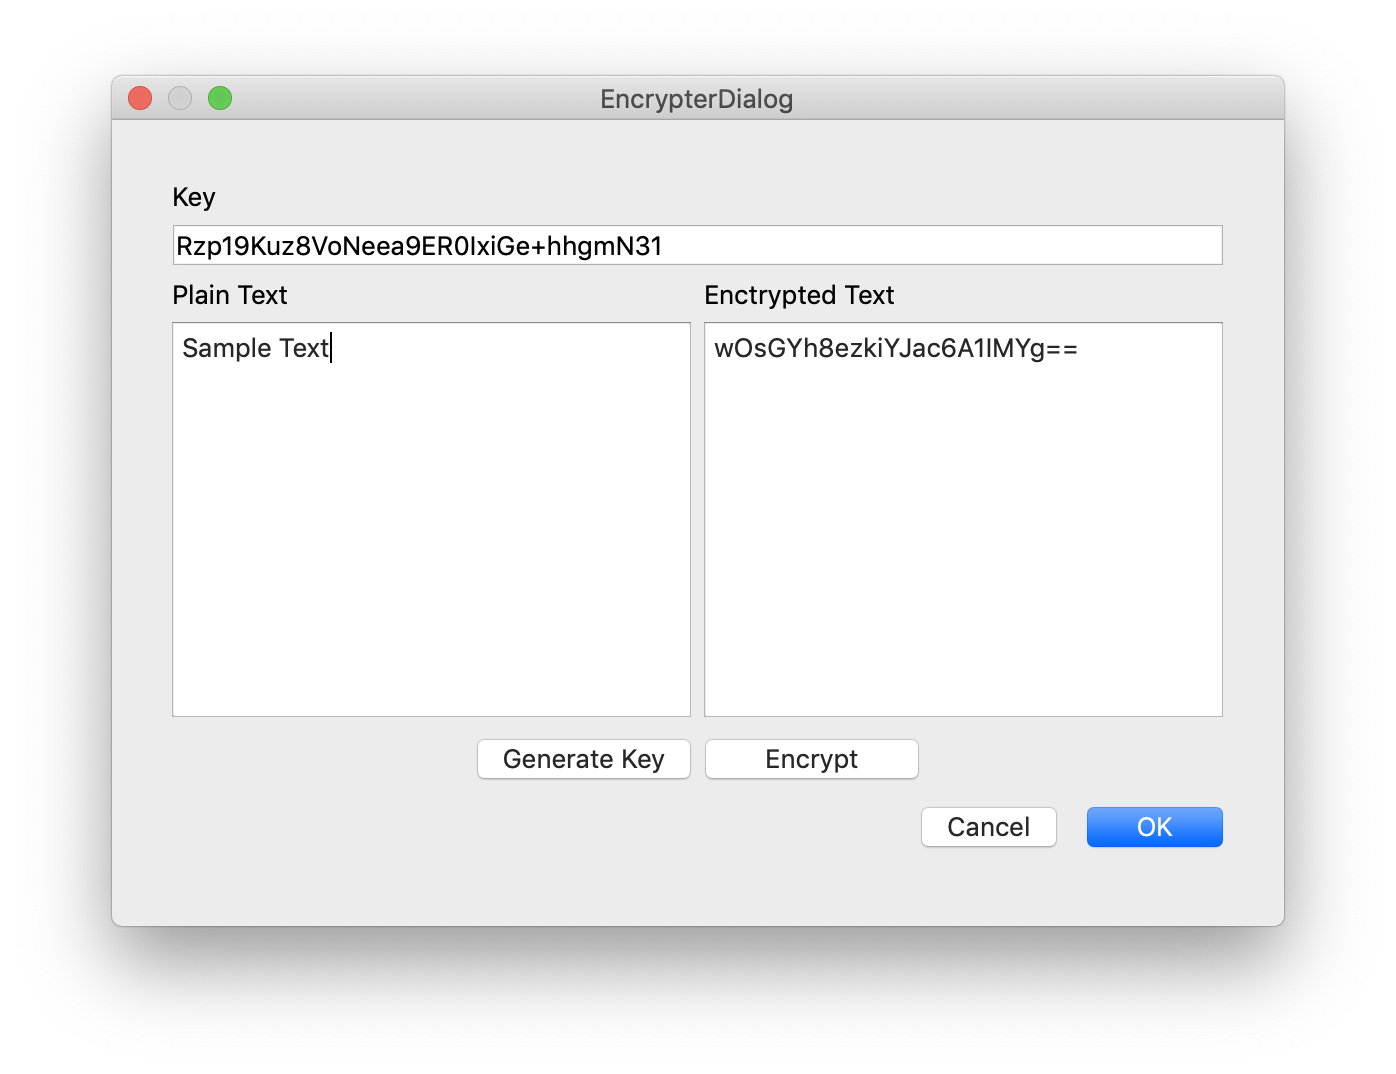
\includegraphics[width = 0.8\textwidth]{encryptor}
\caption{Encryptor Dialog\label{fig:Encryptor Dialog}}
\end{figure} 

\section{Signal and Register Naming}
In practice, we name signals and registers after a certain pattern. For example, a register might be named after \$\{BLOCK\_ABBREVIATION\}\_MAIN\_REG. In this example, the block abbreviation is prepended to the central name MAIN, and a constant string "REG" is appended to the name. The block abbreviation, the what we call given name, and the suffix "REG" are concatenated with an underscore.

The problem is that, if we have to change a system block's abbreviation, then all registers have to be renamed. This introduces more database operations and unreliability. Our solution is simple: we only store the given name in the database. However, the extended name is generated with the naming template and the given name. 

Thus, we designed a NamingTemplate class in which we are able to generate the extended name with the given name, and the other way around. The idea is that we maintain a naming template like \$\{BLOCK\_ABBREVIATION\}\_\$\{GIVEN\_NAME\}\_REG. The naming template contains variables like \$\{Variable\} and constant. The given name variable must always be in the template. To generate the extended name, we simply replace the variables with the abbreviation name of the current system block, and the given name of the current register, which is retrieved from the database. Similarly, we can also generate the given name given an extended name.

To change the naming of signals or registers, we don't have to do anything on the database. We simply make a new naming template and refresh the UI. We designed a very friendly dialog to change the naming template. Users just need to add keywords or constants, and specify a delimiter.

\begin{figure}[htbp]
\centering
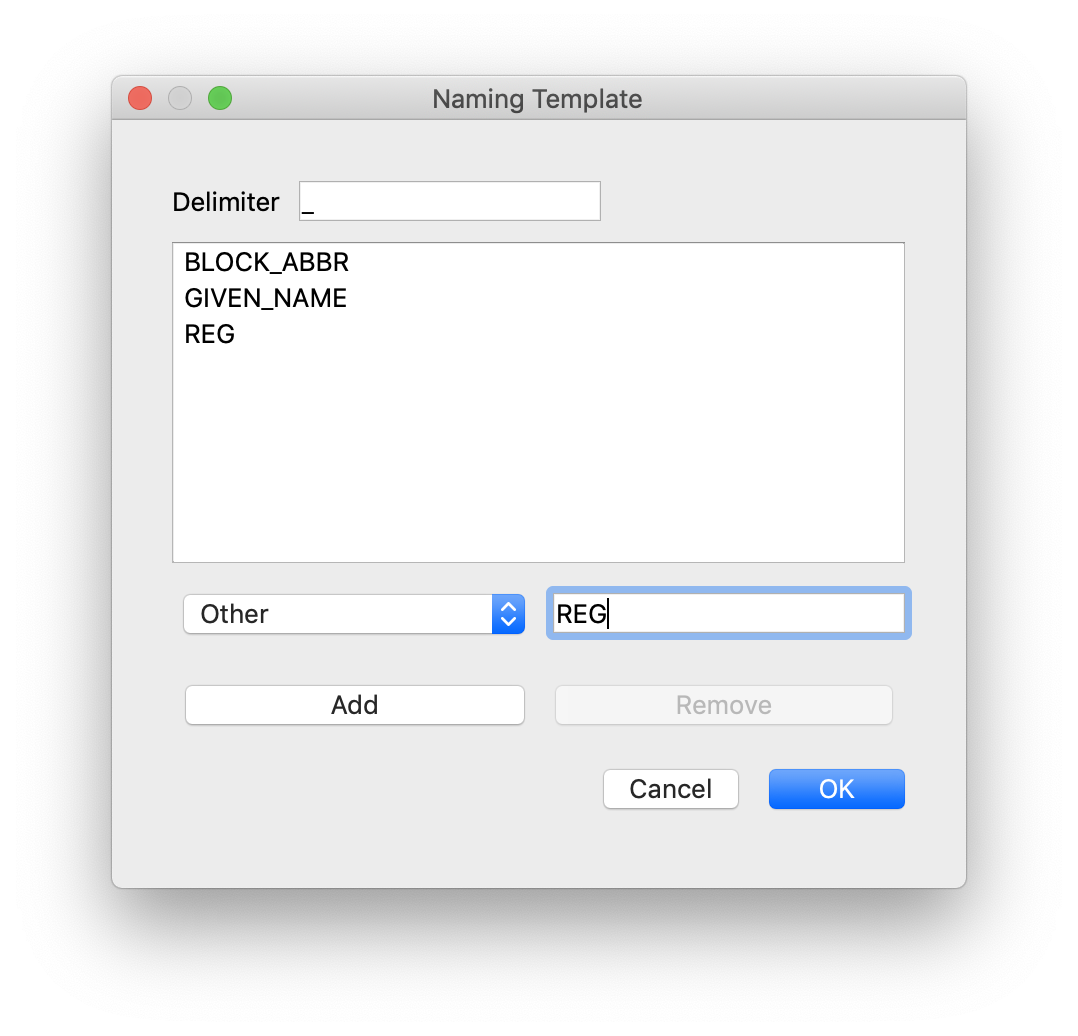
\includegraphics[width = 0.8\textwidth]{namingtemplatedialog}
\caption{Naming Template Dialog\label{fig:Naming Template Dialog}}
\end{figure} 

\section{SPI Interface Generation}
With all the chip definitions and documents, our final goals are generating the SPI configuration interface and a LaTeX documentation. We might want to generate the interface in different languages, so far we only implement VHDL. Despite of this, during design and implement, we already leave flexibility for extensions.

The VHDL SPI interface consists of two files, the interface package, where basic information about the chip is defined, and the interface, where the VHDL interface and behavior is defined. Users can define a package and a interface template with predefined markers. The software will replace the markers with what it generated from the database.

\begin{lstlisting}[language=VHDL]
-- sample VHDL package template
LIBRARY ieee;
  USE ieee.std_logic_1164.all;
  USE ieee.numeric_std.all;
  
PACKAGE interface_package IS

  constant address_width      : integer := 12;
  constant byte_size          : integer := 8;
  constant reg_width           : integer := 8;
  -- FIFO
  constant byte_counter_width : integer := 10;
  constant fifo_size          : integer := 2**byte_counter_width;
  constant packet_size        : integer := 2**byte_size;

   -- REGISTER ADDRESSES
  @PACKAGE_ADDRESSES    -- to be completed by EDA tool

  -- REGISTER_INITIAL VALUES
  @PACKAGE_INITS    -- to be completed by EDA tool
  
END PACKAGE interface_package;
\end{lstlisting}

In the package template there are two makers, one for register address definitions, and the other for initial values definitions for writable registers. Since we allocated each system block a start address, it's easy to infer the address for each register. The initial values of each writable registers are tricky. We have to compute compute initial values for each register bit by looking for the corresponding signal bit it is mapped to, and the initial signal value. Then, the initial value of the registers are obtained by concatenating the initial values of each register bit.

\begin{lstlisting}[language=VHDL]
-- sample VHDL package template
library IEEE;
use IEEE.STD_LOGIC_1164.ALL;
use IEEE.NUMERIC_STD.ALL;

LIBRARY work;
use work.interface_package.ALL;

entity interface is
  generic
  (
    data_width : integer := 12
  );
  port
  (
    resetn                    : in  std_logic;
    clk_main                  : in  std_logic;
    enable                    : in  std_logic;
    
    -- REGISTER SIGNAL PORT DEFINITIONS      
    @PORT_DEFINITIONS
 
  );
end interface;

architecture Behavioral of interface is

  -- INTERNAL SIGNALS FOR INTERFACE FUNCTION
  signal addr_buffer            : std_logic_vector(address_width-1 downto 0);
  signal reg_read_buffer        : std_logic_vector(byte_size-1 downto 0);
  signal byte_ext2asc           : std_logic_vector(byte_size-1 downto 0);
  
  -- INTERNAL SIGNALS NOT CREATED BY THE AUTOMATIC EXPORT
  signal SM_INVERT_FIFO_CLK     : std_logic;  
  signal SM_FIFO_SPI_RESETB     : std_logic;
  signal CHIP_ID_VALUE		: std_logic_vector(16-1 downto 0);
  signal CHIP_REGPAGE_CTRL	: std_logic_vector(2-1 downto 0);

  -- REGISTER DEFINITIONS
  @REGISTER_DEFINITIONS

begin 
  
  reg_write_proc: PROCESS(clk_main, resetn, enable)
  BEGIN
    if resetn = '0' then
      -- Registers
      @REGISTER_INIT

      new_spi_reg_write       <= '0';
    else
      if rising_edge(clk_main) and enable = '1' then
        if current_state = S_DATW and byte_ext2asc_rising = '1' then
          new_spi_reg_write  <= '1';
          case addr_buffer is
            @REG_WRITE_ACCESS

            when others                         => null;
          end case;
        else
          new_spi_reg_write <= '0';
        end if;
      end if;
    end if;
  END PROCESS reg_write_proc;
  
  reg_read_proc: PROCESS(clk_main, resetn, enable)
  BEGIN
    if resetn = '0' then
      reg_read_buffer  <= (others => '0');
      new_spi_reg_read            <= '0';
    else
      if rising_edge(clk_main) and enable = '1' then
        if current_state = S_DATR then
          new_spi_reg_read        <= '1';
          case addr_buffer is
            @REG_READ_ACCESS

            when others                         => null;
          end case;
        else 
          new_spi_reg_read        <= '0';
          reg_read_buffer         <= (others => '0');
        end if;
      end if;
    end if;
  END PROCESS reg_read_proc;
  
  @SIGNAL_ASSIGNMENTS
  
end Behavioral;
\end{lstlisting}

The interface is more complex. It consists of two code blocks, the entity definition, and the behavioral definition. In the entity definition, the software shall complete the port definitions. All port signals should be included. Then, in the behavioral definition, the software first complete the register definitions. After after clock, the interface should do read or write process. It reads data from external. According to the address buffer, the data should be written to a certain register. Otherwise it reads data from a certain register, and write to external. Finally, the software should assign values. In case of a read-only register, the software shall assign to it values from the signals it is mapped to. In case of a writable register, the software shall assign values to the signals it is mapped to. Paged registers are dealt with in a special way.

We designed a VHDLGenerator class. The generation process of the interface is described as the following pseudo code. Generation of the package follows the same structure.

\begin{lstlisting}[language=C++]
QString VHDLGenerator::generate_interface() const
{
    QString ports,
            register_definitions, register_inits,
            register_write_accesses, register_read_accesses,
            readonly_register_assignments,
            control_signal_assignments,
            paged_register_assignments;
            
    QVector<QString> blocks = read_system_blocks();
    for (const auto& block : blocks)
    {
        QVector<QString> interface_block = generate_interface_block(block);
        ports += interface_block[0];
        register_definitions += interface_block[1];
        register_inits += interface_block[2];
        register_write_accesses += interface_block[3];
        register_read_accesses += interface_block[4];
        readonly_register_assignments += interface_block[5];
        control_signal_assignments += interface_block[6];
        paged_register_assignments += interface_block[7];
    }
    QString interface = get_interface_template();
    interface.replace(marker_ports, ports);
    interface.replace(marker_register_definitions, register_definitions);
    interface.replace(marker_register_init, register_inits);
    interface.replace(marker_register_write, register_write_accesses);
    interface.replace(marker_register_read, register_read_accesse);
    interface.replace(marker_signal_assignment, signal_assignments);
      
    return interface;
}

QVector<QString> VHDLGenerator::generate_interface_block(block) const
{
    QVector<QString> signals = read_signals(block);
    QVector<QString> registers = read_registers(block);
    QString ports,
            register_definitions, register_inits,
            register_write_accesses, register_read_accesses,
            readonly_register_assignments, 
            control_signal_assignments, 
            paged_register_assignments;
            
    for (const auto& register : registers)
    {
        register_definitions += generate_register_definition(register);
        register_read_accesses += generate_reading_register(register);
        if (writable(register))
        {
            register_inits += generate_initializing_register(register);
            register_write_accesses += generate_writing_register(register);
        }
        else
        {
            readonly_register_assignments += generate_assigning_value_to_readonly_register(register);
        }
        if (paged_register(register))
            paged_register_assignments += generate_assigning_value_to_paged_register(register);
    }
    
    for (const auto& signal : signals)
    {
        if (port_signal(signal)) 
            ports += generate_port_definition(signal);
        if (control_signal(signal)) 
            control_signal_assignments += generate_assigning_value_to_constrol_signal(signal);
    }
    
    return {ports,
            register_definitions, register_inits,
            register_write_accesses, register_read_accesses,
            readonly_register_assignments, 
            control_signal_assignments, 
            paged_register_assignments};
}
\end{lstlisting}

We made a SPIGenerationDialog class for users to configure the generation. The designing pattern is similar to the previous editor dialogs. Since the generated code must be directly usable, we have to make sure there are no errors. Sanity checks must be done.

\begin{figure}[htbp]
\centering
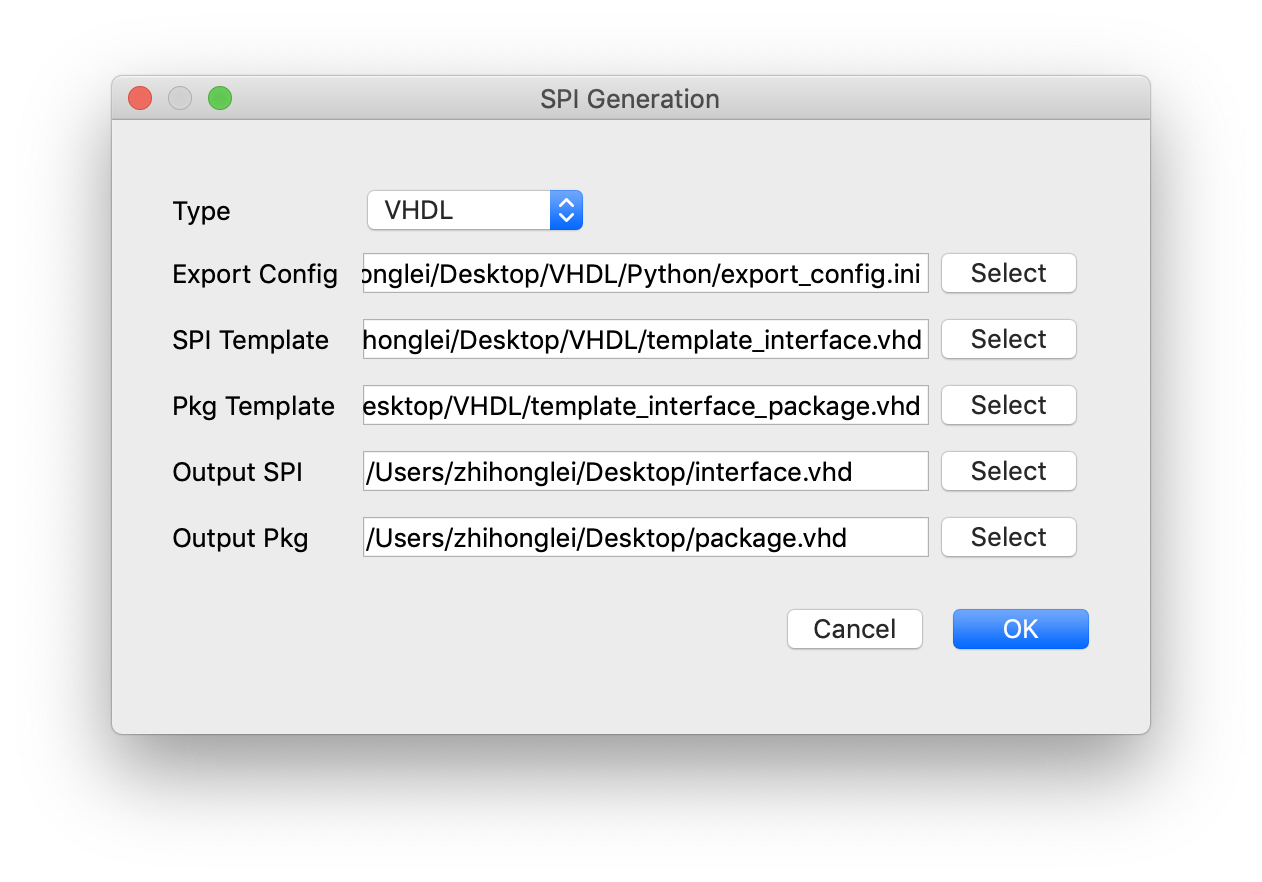
\includegraphics[width = 0.8\textwidth]{spigenerationdialog}
\caption{SPI Generation Dialog\label{fig:SPI Generation Dialog}}
\end{figure} 

\section{Document Generation}
So far chip designers have added documents to each system block, register and signal, and also the chip itself as well. The software will compose them and generate a complete documentation.

The documentation is well structured. Thus, we designed a documentation generator following this structure.

\begin{figure}[htbp]
\centering
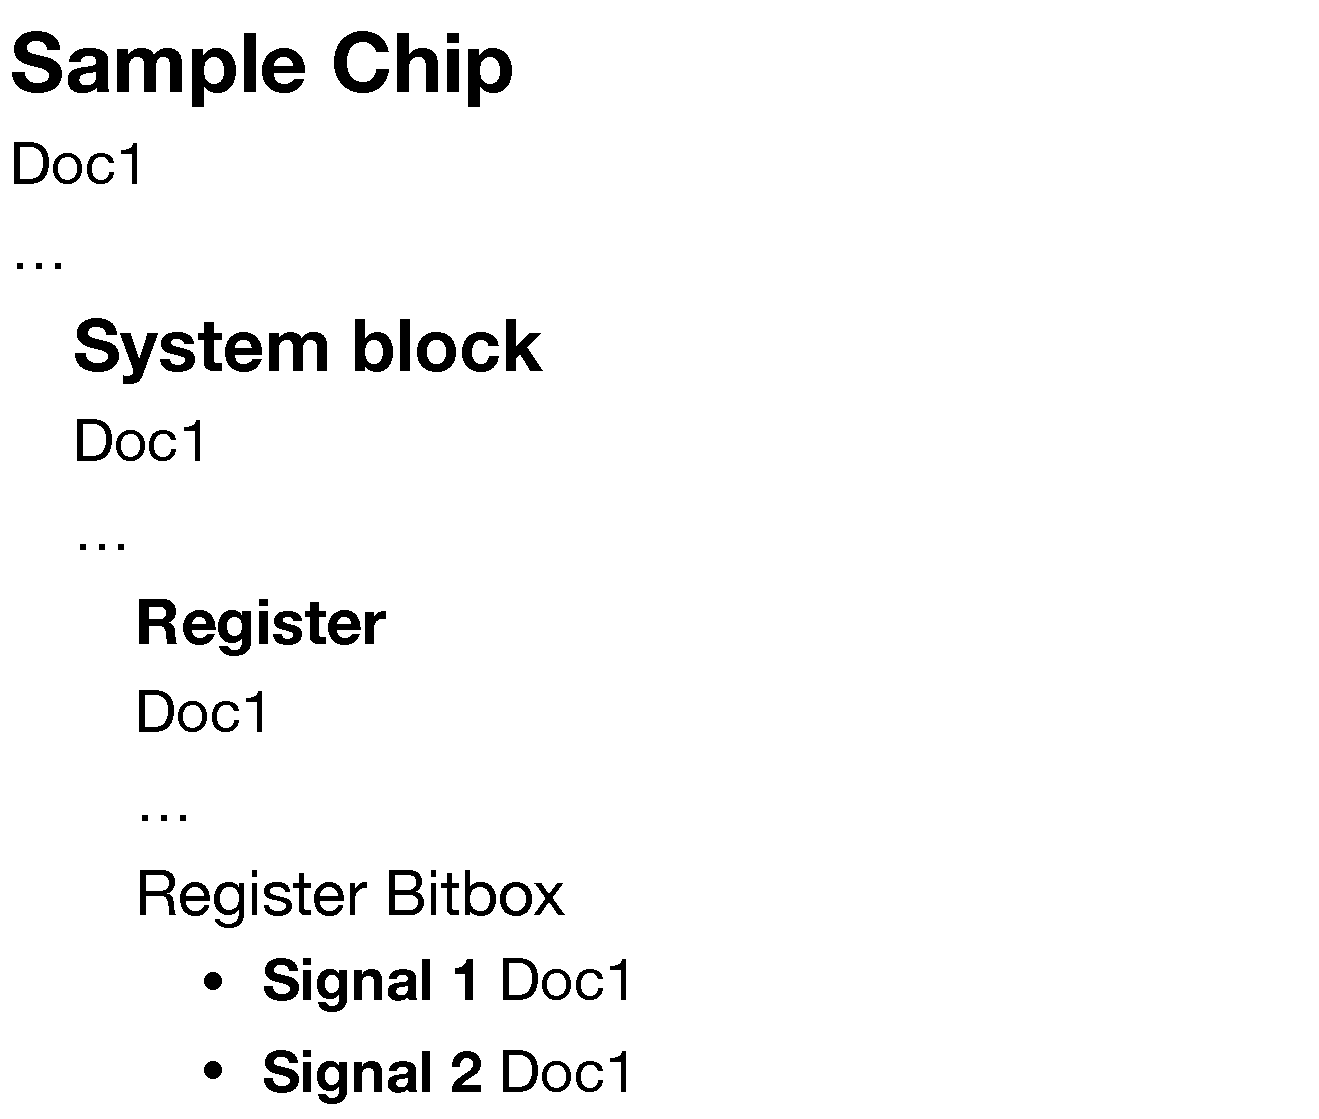
\includegraphics[width = 0.8\textwidth]{docstructure}
\caption{Structure of the Documentation\label{fig:Structure of the Documentation}}
\end{figure} 

\begin{lstlisting}[language=C++]
// document_generator.h

// functions to generate the LaTeX documentation
// parameters are omitted
QString generate_tex_document();
QString generate_chip_level_tex_document();
QString generate_block_level_tex_document();
QString generate_register_level_tex_document();
QString generate_register_bit_table_tex();
QString generate_register_signal_bullets_tex();

// static functions to generate single documents into LaTeX
static QString generate_text_tex(const QString& text);
static QString generate_image_tex(const QString& caption, const QString& width, const QString& path);
static QString generate_table_tex(const QString& caption, const QVector<QVector<QString> >& cells);
\end{lstlisting}

In previous sections, we have introduced a document preview for the document editor.  It is basically a web browser rendering HTML web page with LaTeX source code with the help of MathJax. Since the software is already able to display a single document, why not implement a full documentation generation function in HTML format, and make a preview of the complete documentation?

Inspired by this, we implemented the HTML generation functions in a similar way to LaTeX. We can generate a full HTML documentation, and let the software display it. Users can also choose to generate the HTML document. In some cases it would be a better choice than LaTeX, for example, if the Chair of IAS wants to make an internal wiki.

\begin{figure}[htbp]
\centering
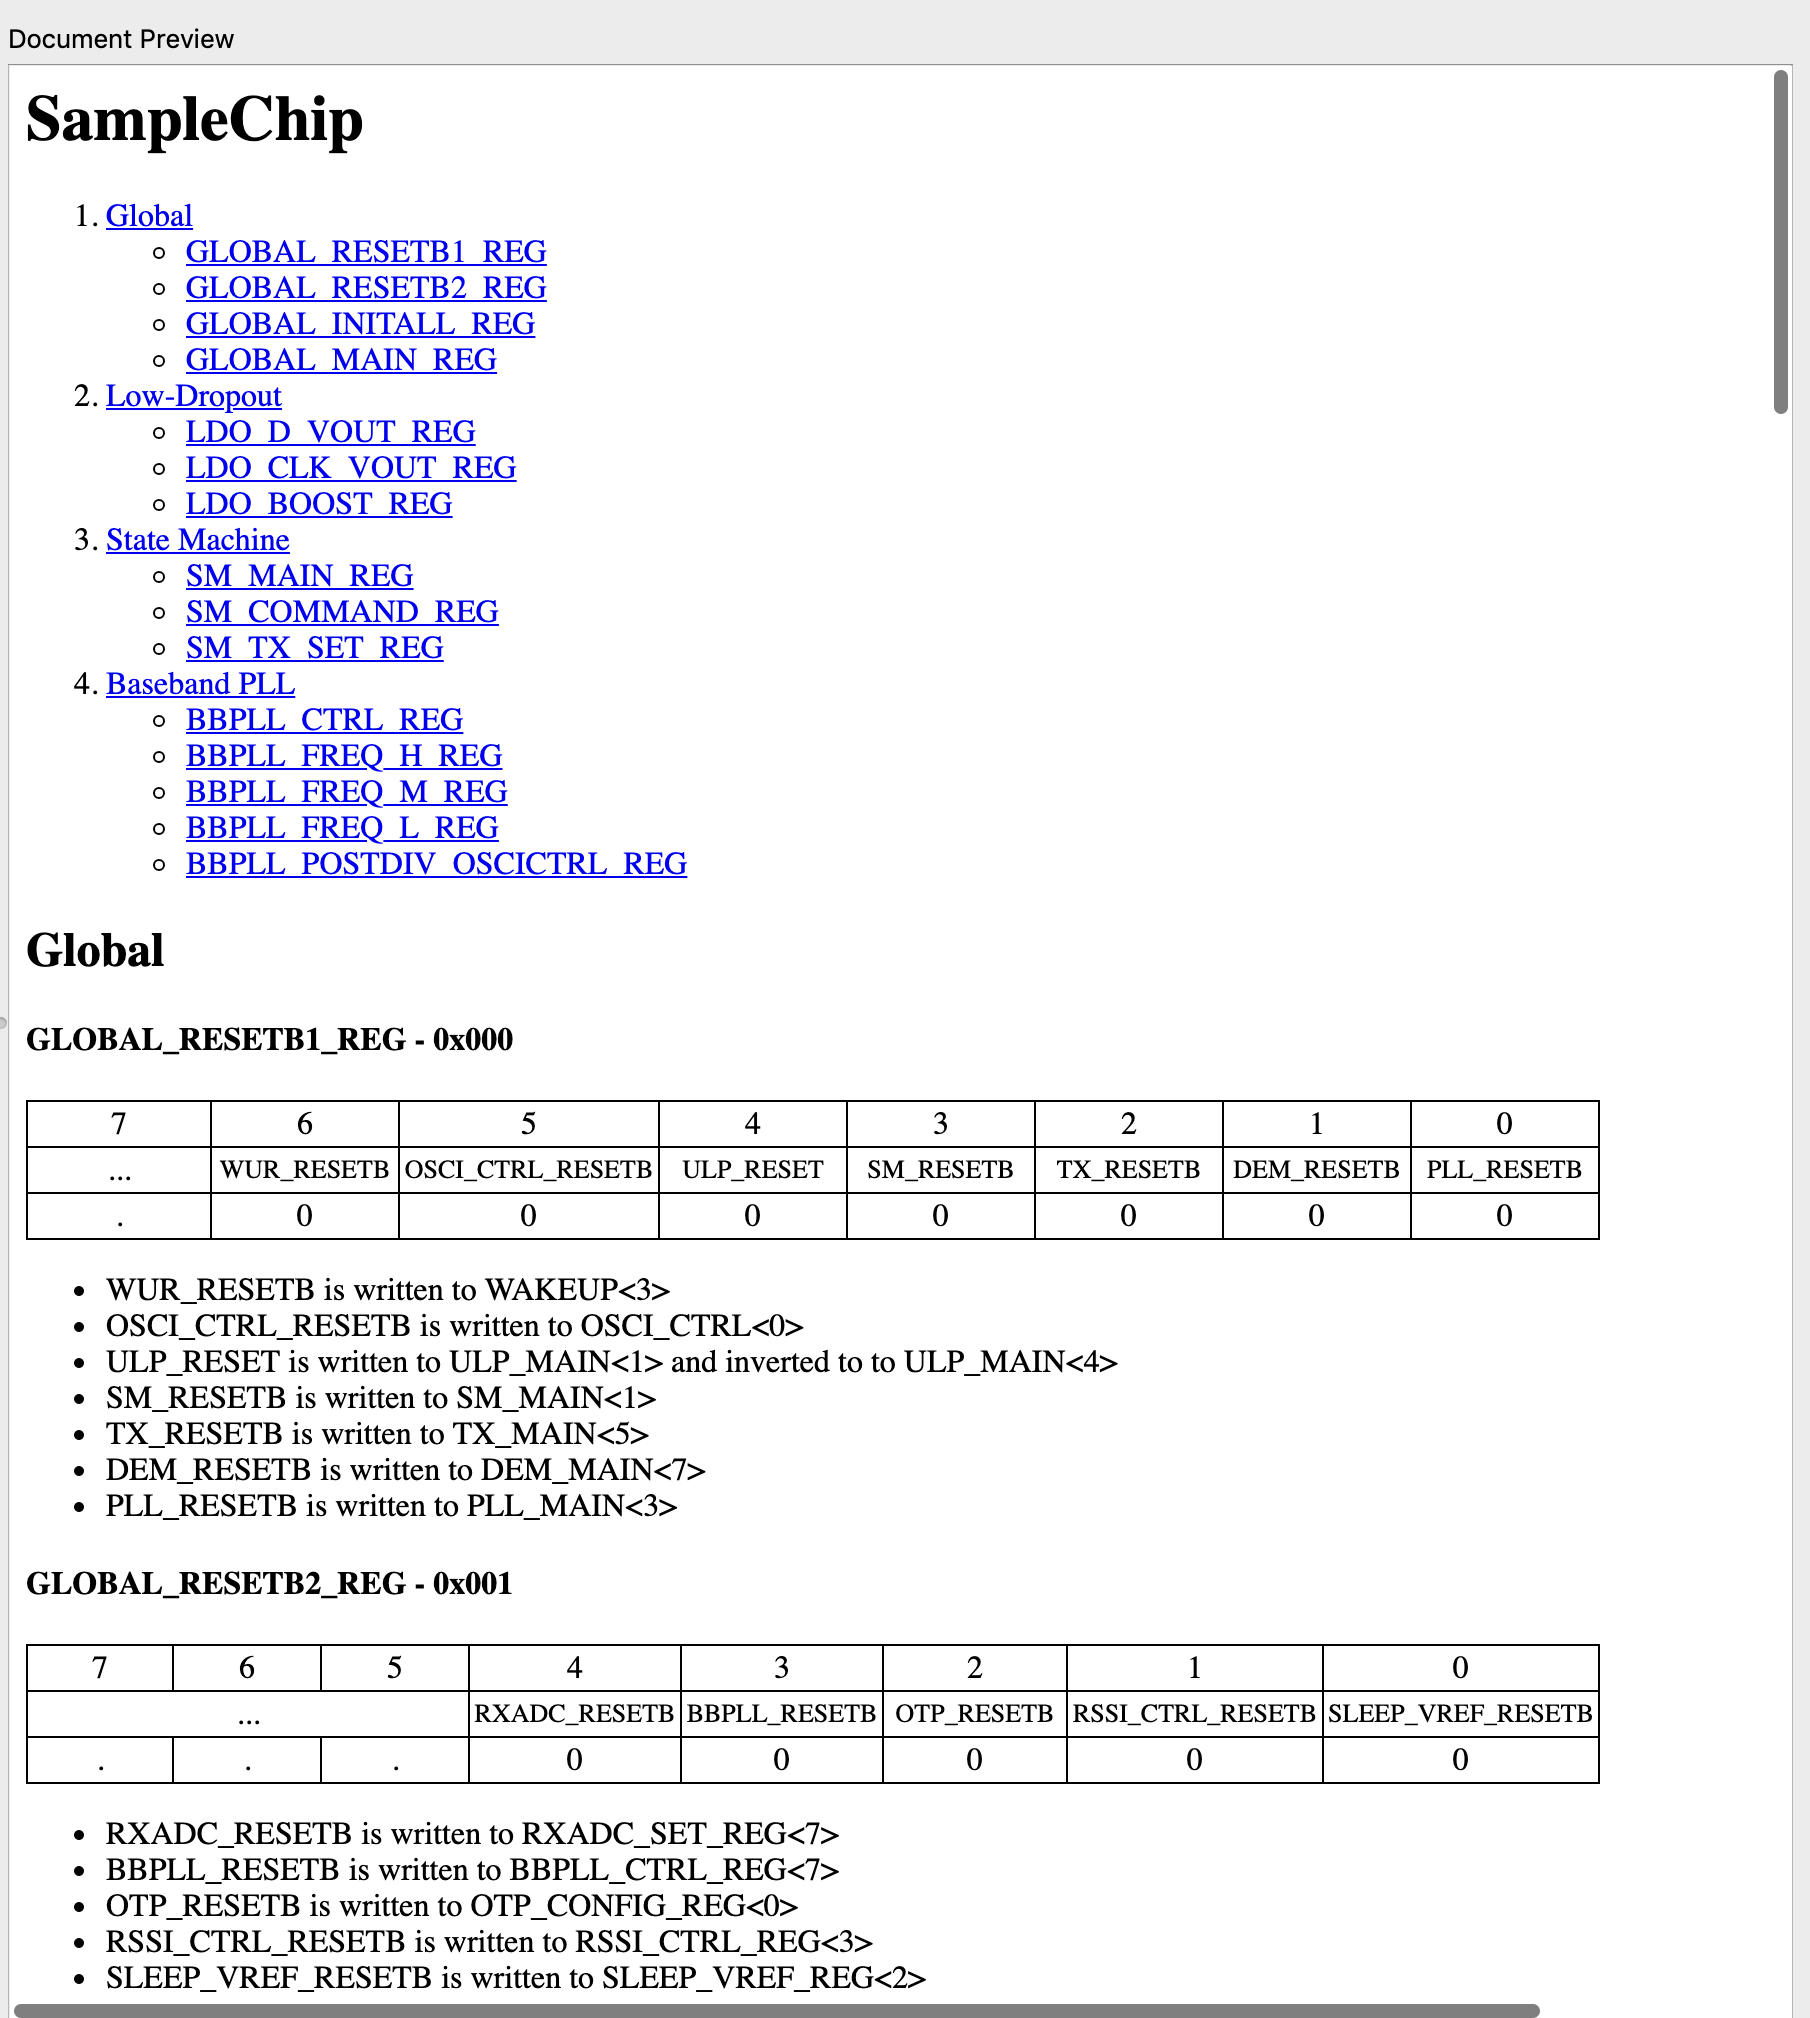
\includegraphics[width = \textwidth]{htmldocexample}
\caption{Document Preview in HTML Format\label{fig:Document Preview in HTML Format}}
\end{figure} 

Similarly, we created a DocumentGenerationDialog for users to select the document format, configure the documentation and select which system blocks they want to generate.

\begin{figure}[htbp]
\centering
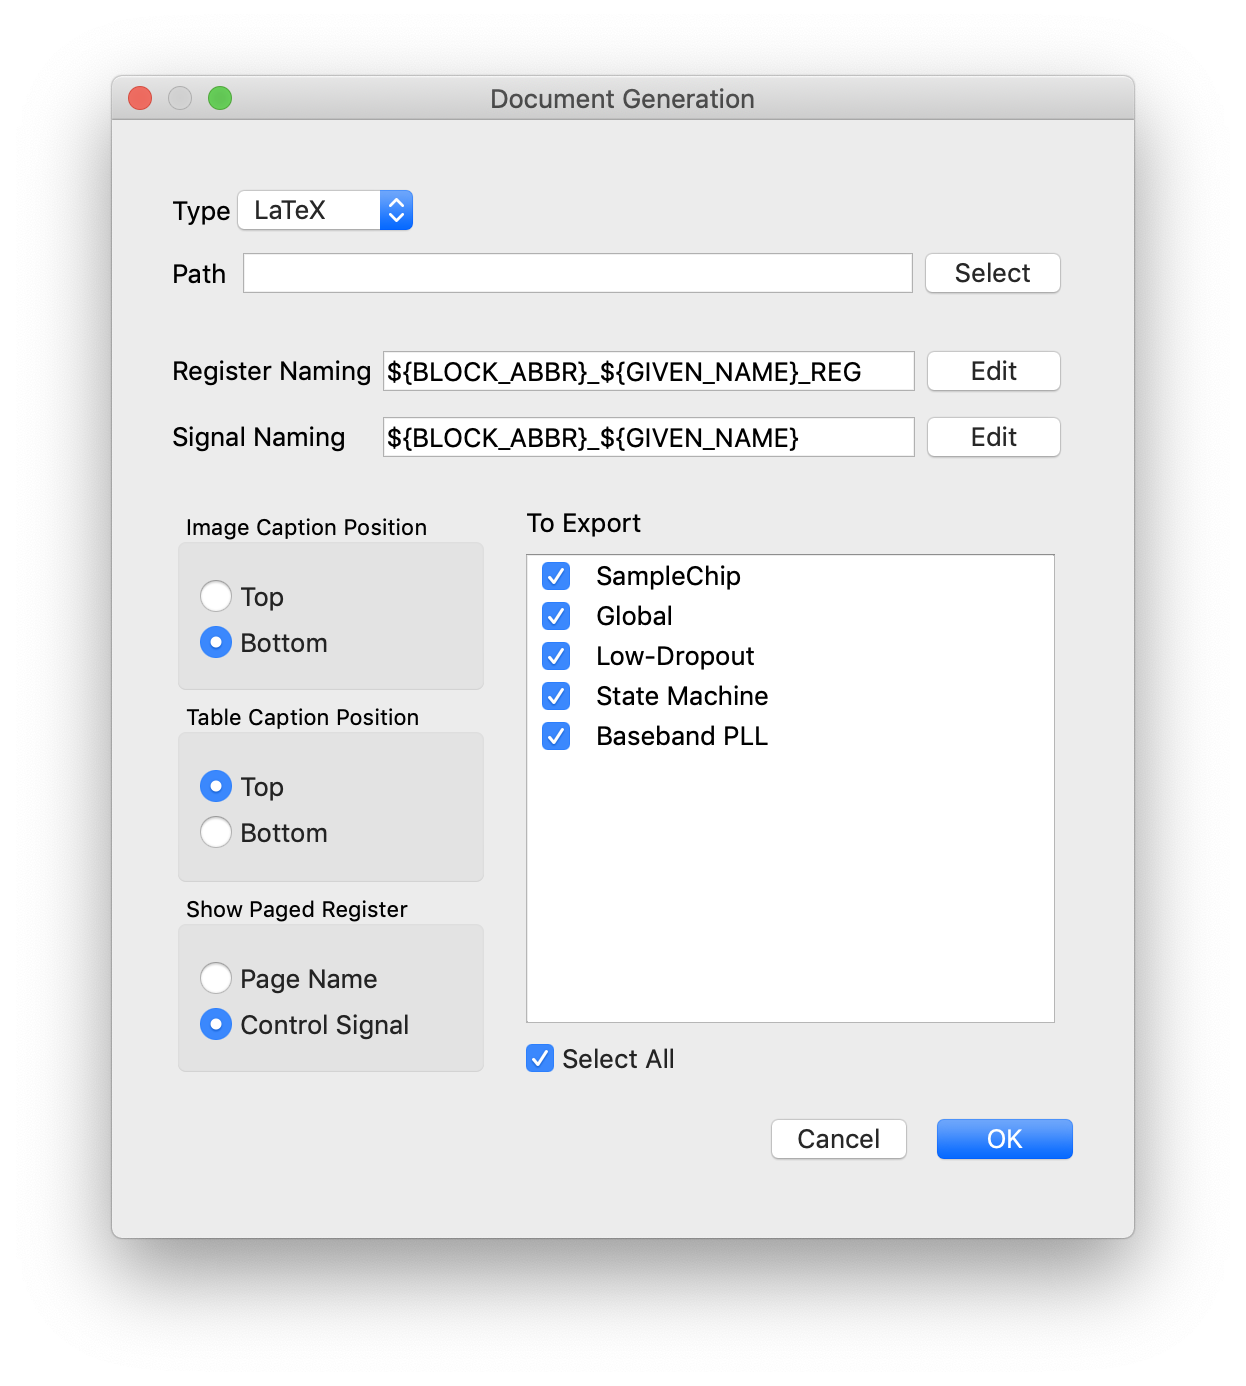
\includegraphics[width = 0.8\textwidth]{docgenerationdialog}
\caption{Documentation Generation Dialog\label{fig:Documentation Generation Dialog}}
\end{figure} 
